\documentclass[10pt]{article}
\usepackage[T1]{fontenc}
\usepackage[utf8]{inputenc}
% \usepackage{lmodern}
%\usepackage[adobe-utopia,uppercase=upright,greeklowercase=upright]{mathdesign}
\usepackage[adobe-utopia]{mathdesign}
%\usepackage{minionpro}
% \usepackage{pifont}
% \usepackage{amssymb}
\usepackage{amsmath}
\usepackage[francais]{babel}
% \usepackage[francais]{varioref}
\usepackage[dvips]{graphicx}

\usepackage{framed}
\usepackage[normalem]{ulem}
\usepackage{fancyhdr}
\usepackage{titlesec}
\usepackage{vmargin}
\usepackage{longtable}

\usepackage{ifthen}


%\usepackage{epsfig}
\usepackage{subfig}

\usepackage{multirow}
\usepackage{multicol} % Portions de texte en colonnes
\usepackage{flafter}%floatants après la référence



\usepackage{color}
\usepackage{colortbl}


\definecolor{gris25}{gray}{0.75}
\definecolor{bleu}{RGB}{18,33,98}
\definecolor{bleuf}{RGB}{42,94,171}
\definecolor{bleuc}{RGB}{231,239,247}
\definecolor{rougef}{RGB}{185,18,27}
\definecolor{rougec}{RGB}{255,230,231}
\definecolor{vertf}{RGB}{103,126,82}
\definecolor{vertc}{RGB}{220,255,191}

\newenvironment{rem}[1][\hsize]%
{%
    \def\FrameCommand
    {%
\rotatebox{90}{\textit{\textsf{Remarque}}} 
        {\color{bleuf}\vrule width 3pt}%
        \hspace{0pt}%must no space.
        \fboxsep=\FrameSep\colorbox{bleuc}%
    }%
    \MakeFramed{\hsize#1\advance\hsize-\width\FrameRestore}%
}%
{\endMakeFramed}%


\newenvironment{savoir}[1][\hsize]%
{%
    \def\FrameCommand
    {%
\rotatebox{90}{\textit{\textsf{Savoir}}} 
        {\color{bleuf}\vrule width 3pt}%
        \hspace{0pt}%must no space.
        \fboxsep=\FrameSep\colorbox{bleuc}%
    }%
    \MakeFramed{\hsize#1\advance\hsize-\width\FrameRestore}%
}%
{\endMakeFramed}%

\newenvironment{prob}[1][\hsize]%
{%
    \def\FrameCommand%
    {%
\rotatebox{90}{\textit{\textsf{ Problématique}}} 
        {\color{rougef}\vrule width 3pt}%
        \hspace{0pt}%must no space.
        \fboxsep=\FrameSep\colorbox{rougec}%
    }%
    \MakeFramed{\hsize#1\advance\hsize-\width\FrameRestore}%
}%
{\endMakeFramed}%

\newenvironment{obj}[1][\hsize]%
{%
    \def\FrameCommand%
    {%
\rotatebox{90}{\textit{\textsf{ $\;$}}} 
        {\color{rougef}\vrule width 3pt}%
        \hspace{0pt}%must no space.
        \fboxsep=\FrameSep\colorbox{rougec}%
    }%
    \MakeFramed{\hsize#1\advance\hsize-\width\FrameRestore}%
}%
{\endMakeFramed}%

\newenvironment{defi}[1][\hsize]%
{%
    \def\FrameCommand%
    {%
\rotatebox{90}{\textit{\textsf{Définition\\}}} 
        {\color{bleuf}\vrule width 3pt}%
        \hspace{0pt}%must no space.
        \fboxsep=\FrameSep\colorbox{bleuc}%
    }%
    \MakeFramed{\hsize#1\advance\hsize-\width\FrameRestore}%
}%
{\endMakeFramed}%


\newenvironment{hypo}[1][\hsize]%
{%
    \def\FrameCommand%
    {%
\rotatebox{90}{\textit{\textsf{Hypothèse\\}}} 
        {\color{bleuf}\vrule width 3pt}%
        \hspace{0pt}%must no space.
        \fboxsep=\FrameSep\colorbox{bleuc}%
    }%
    \MakeFramed{\hsize#1\advance\hsize-\width\FrameRestore}%
}%
{\endMakeFramed}%


\newenvironment{prop}[1][\hsize]%
{%
    \def\FrameCommand%
    {%
\rotatebox{90}{\textit{\textsf{Propriété\\}}} 
        {\color{bleuf}\vrule width 3pt}%
        \hspace{0pt}%must no space.
        \fboxsep=\FrameSep\colorbox{bleuc}%
    }%
    \MakeFramed{\hsize#1\advance\hsize-\width\FrameRestore}%
}%
{\endMakeFramed}%

\newenvironment{props}[1][\hsize]%
{%
    \def\FrameCommand%
    {%
\rotatebox{90}{\textit{\textsf{Propriétés\\}}} 
        {\color{bleuf}\vrule width 3pt}%
        \hspace{0pt}%must no space.
        \fboxsep=\FrameSep\colorbox{bleuc}%
    }%
    \MakeFramed{\hsize#1\advance\hsize-\width\FrameRestore}%
}%
{\endMakeFramed}%

\newenvironment{exemple}[1][\hsize]%
{%
    \def\FrameCommand%
    {%
\rotatebox{90}{\textit{\textsf{Exemple\\}}} 
        {\color{vertf}\vrule width 3pt}%
        \hspace{0pt}%must no space.
        \fboxsep=\FrameSep\colorbox{vertc}%
    }%
    \MakeFramed{\hsize#1\advance\hsize-\width\FrameRestore}%
}%
{\endMakeFramed}%

\newenvironment{resultat}[1][\hsize]%
{%
    \def\FrameCommand%
    {%
\rotatebox{90}{\textit{\textsf{Résultat\\}}} 
        {\color{rougef}\vrule width 3pt}%
        \hspace{0pt}%must no space.
        \fboxsep=\FrameSep\colorbox{rougec}%
    }%
    \MakeFramed{\hsize#1\advance\hsize-\width\FrameRestore}%
}%
{\endMakeFramed}%

\newenvironment{methode}[1][\hsize]%
{%
    \def\FrameCommand%
    {%
\rotatebox{90}{\textit{\textsf{Méthode\\}}} 
        {\color{rougef}\vrule width 3pt}%
        \hspace{0pt}%must no space.
        \fboxsep=\FrameSep\colorbox{rougec}%
    }%
    \MakeFramed{\hsize#1\advance\hsize-\width\FrameRestore}%
}%
{\endMakeFramed}%

\newenvironment{theo}[1][\hsize]%
{%
    \def\FrameCommand%
    {%
\rotatebox{90}{\textit{\textsf{Théorème\\}}} 
        {\color{rougef}\vrule width 3pt}%
        \hspace{0pt}%must no space.
        \fboxsep=\FrameSep\colorbox{rougec}%
    }%
    \MakeFramed{\hsize#1\advance\hsize-\width\FrameRestore}%
}%
{\endMakeFramed}%

\newenvironment{warn}[1][\hsize]%
{%
    \def\FrameCommand%
    {%
\rotatebox{90}{\textit{\textsf{Attention\\}}} 
        {\color{rougef}\vrule width 3pt}%
        \hspace{0pt}%must no space.
        \fboxsep=\FrameSep\colorbox{rougec}%
    }%
    \MakeFramed{\hsize#1\advance\hsize-\width\FrameRestore}%
}%
{\endMakeFramed}%

% \usepackage{pstricks}
%\usepackage{minitoc}
% \setcounter{minitocdepth}{4}

\setcounter{tocdepth}{2}

% \mtcselectlanguage{french} 

%\usepackage{draftcopy}% "Brouillon"
% \usepackage{floatflt}
\usepackage{psfrag}
%\usepackage{listings} % Permet d'insérer du code de programmation
\renewcommand{\baselinestretch}{1.2}

% Changer la numérotation des figures :
% ------------------------------------
% \makeatletter
% \renewcommand{\thefigure}{\ifnum \c@section>\z@ \thesection.\fi
%  \@arabic\c@figure}
% \@addtoreset{figure}{section}
% \makeatother
 


%%%%%%%%%%%%
% Définition des vecteurs %
%%%%%%%%%%%%
 \newcommand{\vect}[1]{\overrightarrow{#1}}

%%%%%%%%%%%%
% Définition des torseusr %
%%%%%%%%%%%%

 \newcommand{\torseur}[1]{%
\left\{{#1}\right\}
}

\newcommand{\torseurcin}[3]{%
\left\{\mathcal{#1} \left(#2/#3 \right) \right\}
}

\newcommand{\torseurstat}[3]{%
\left\{\mathcal{#1} \left(#2\rightarrow #3 \right) \right\}
}

 \newcommand{\torseurc}[8]{%
%\left\{#1 \right\}=
\left\{
{#1}
\right\}
 = 
\left\{%
\begin{array}{cc}%
{#2} & {#5}\\%
{#3} & {#6}\\%
{#4} & {#7}\\%
\end{array}%
\right\}_{#8}%
}

 \newcommand{\torseurcol}[7]{
\left\{%
\begin{array}{cc}%
{#1} & {#4}\\%
{#2} & {#5}\\%
{#3} & {#6}\\%
\end{array}%
\right\}_{#7}%
}

 \newcommand{\torseurl}[3]{%
%\left\{\mathcal{#1}\right\}_{#2}=%
\left\{%
\begin{array}{l}%
{#1} \\%
{#2} %
\end{array}%
\right\}_{#3}%
}

 \newcommand{\vectv}[3]{%
\vect{V\left( {#1} \in {#2}/{#3}\right)}
}


\newcommand{\vectf}[2]{%
\vect{R\left( {#1} \rightarrow {#2}\right)}
}

\newcommand{\vectm}[3]{%
\vect{\mathcal{M}\left( {#1}, {#2} \rightarrow {#3}\right)}
}


 \newcommand{\vectg}[3]{%
\vect{\Gamma \left( {#1} \in {#2}/{#3}\right)}
}

 \newcommand{\vecto}[2]{%
\vect{\Omega\left( {#1}/{#2}\right)}
}
% }$$\left\{\mathcal{#1} \right\}_{#2} =%
% \left\{%
% \begin{array}{c}%
%  #3 \\%
%  #4 %
% \end{array}%
% \right\}_{#5}}

%  ------------------------------------------
% | Modification du formatage des sections : | 
%  ------------------------------------------

% Grands titres :
% ---------------

\newcommand{\titre}[1]{%
\begin{center}
      \bigskip
      \rule{\textwidth}{1pt}
      \par\vspace{0.1cm}
      
      \textbf{\large #1}
      \par\rule{\textwidth}{1pt}
    \end{center}
    \bigskip
  }

% Supprime le numéro du chapitre dans la numérotation des sections:
% -----------------------------------------------------------------
\makeatletter
\renewcommand{\thesection}{\@arabic\c@section}
\makeatother


% \titleformat{\chapter}[display]
% {\normalfont\Large\filcenter}
% {}
% {1pc}
% {\titlerule[1pt]
%   \vspace{1pc}%
%   \Huge}[\vspace{1ex}%
% \titlerule]


%%%% Chapitres Comme PY Pechard %%%%%%%%%
% numéro du chapitre
\DeclareFixedFont{\chapnumfont}{OT1}{phv}{b}{n}{80pt}
% pour le mot « Chapitre »
\DeclareFixedFont{\chapchapfont}{OT1}{phv}{m}{it}{40pt}
% pour le titre
\DeclareFixedFont{\chaptitfont}{T1}{phv}{b}{n}{25pt}

\definecolor{gris}{gray}{0.75}
\titleformat{\chapter}[display]%
	{\sffamily}%
	{\filleft\chapchapfont\color{gris}\chaptertitlename\
	\\
	\vspace{12pt}
	\chapnumfont\thechapter}%
	{16pt}%
	{\filleft\chaptitfont}%
	[\vspace{6pt}\titlerule\titlerule\titlerule]

%%%%  Fin Chapitres Comme PY Pechard %%%%%%%%%


% Section, subsection, subsubsection sans serifs :
% % ----------------------------------------------

% \makeatletter
% \renewcommand{\section}{\@startsection{section}{0}{0mm}%
% {\baselineskip}{.3\baselineskip}%
% {\normalfont\sffamily\Large\textbf}}%
% \makeatother

\makeatletter
\renewcommand{\@seccntformat}[1]{{\textcolor{bleu}{\csname
the#1\endcsname}\hspace{0.5em}}}
\makeatother

\makeatletter
\renewcommand{\section}{\@startsection{section}{1}{\z@}%
                       {-4ex \@plus -1ex \@minus -.4ex}%
                       {1ex \@plus.2ex }%
                       {\normalfont\Large\sffamily\bfseries}}%
\makeatother
 
\makeatletter
\renewcommand{\subsection}{\@startsection {subsection}{2}{\z@}
                          {-3ex \@plus -0.1ex \@minus -.4ex}%
                          {0.5ex \@plus.2ex }%
                          {\normalfont\large\sffamily\bfseries}}
\makeatother
 
\makeatletter
\renewcommand{\subsubsection}{\@startsection {subsubsection}{3}{\z@}
                          {-2ex \@plus -0.1ex \@minus -.2ex}%
                          {0.2ex \@plus.2ex }%
                          {\normalfont\large\sffamily\bfseries}}
\makeatother
 
\makeatletter             
\renewcommand{\paragraph}{\@startsection{paragraph}{4}{\z@}%
                                    {-2ex \@plus-.2ex \@minus .2ex}%
                                    {0.1ex}%               
{\normalfont\sffamily\bfseries}}
\makeatother
 
\makeatletter
\renewcommand{\subparagraph}{\@startsection{subparagraph}{5}{\z@}%
                                       {-2ex \@plus-.1ex \@minus .2ex}%
                                       {0.1ex}%
				    {\normalfont\normalsize\sffamily\bfseries}}
\makeatletter
% \makeatletter
% \renewcommand{\subsection}{\@startsection{subsection}{1}{2mm}%
% {\baselineskip}{.3\baselineskip}%
% {\normalfont\sffamily\large\textbf}}%
% \makeatother
% 
% \makeatletter
% \renewcommand{\subsubsection}{\@startsection{subsubsection}{2}{4mm}%
% {\baselineskip}{.15\baselineskip}%
% {\normalfont\sffamily\large\textbf}}%
% \makeatother
% 
% \makeatletter
% \renewcommand{\paragraph}{\@startsection{paragraph}{3}{6mm}%
% {\baselineskip}{.15\baselineskip}%
% {\normalfont\sffamily\large\textbf}}%
% \makeatother
 
\setcounter{secnumdepth}{4}


%  --------
% | Marges |
%  --------


% \setmarginsrb{2.5cm}{1.5cm}{2.5cm}{2cm}{1cm}{1cm}{1cm}{1cm}
\setmarginsrb{1.5cm}{1cm}{1cm}{1.5cm}{1cm}{1cm}{1cm}{1cm}

% Changer les marges localement :
% -----------------------------
\newenvironment{changemargin}[2]{\begin{list}{}{%
\setlength{\topsep}{0pt}%
\setlength{\leftmargin}{0pt}%
\setlength{\rightmargin}{0pt}%
\setlength{\listparindent}{\parindent}%
\setlength{\itemindent}{\parindent}%
\setlength{\parsep}{0pt plus 1pt}%
\addtolength{\leftmargin}{#1}%
\addtolength{\rightmargin}{#2}%
}\item }{\end{list}}



\usepackage{pst-solides3d}
\usepackage{titletoc}
\titlecontents{chapter}[+3pc]
  {\addvspace{10pt}\sffamily\bfseries}
{\contentslabel[{\pscirclebox[fillstyle=solid,fillcolor=gray!25,
linecolor=gray!25,framesep=4pt]{\textcolor{white}{\thecontentslabel}}}]{2.5pc}}
  {}
  {\dotfill \normalfont\thecontentspage\ }

\titlecontents{section}[3pc]
  {\addvspace{2pt}\sffamily}
  {\contentslabel[\thecontentslabel]{1.8pc}}
  {}
  {\dotfill \normalfont\thecontentspage\ }

\titlecontents{subsection}[5pc]
  {\addvspace{2pt}\sffamily}
  {\contentslabel[\thecontentslabel]{1.8pc}}
  {}
  {\dotfill \normalfont\thecontentspage\ }

\titlecontents{subsubsection}[8pc]
  {\addvspace{2pt}\sffamily}
  {\contentslabel[\thecontentslabel]{3pc}}
  {}
  {\dotfill \normalfont\thecontentspage\ }
%{\;\titlerule\;\normalfont\thecontentspage\ }

\titlecontents{paragraph}[9pc]
  {\addvspace{2pt}\sffamily}
  {\contentslabel[\thecontentslabel]{3.5pc}}
  {}
  {\dotfill \normalfont\thecontentspage\ }



%\usepackage{algorithm}
%\usepackage{algorithmic}
\usepackage[french]{algorithm2e}

\SetKwBlock{Fonction}{Début Fonction}{Fin Fonction}
\SetKwComment{Comment}{start}{end}
% Python sources

\usepackage{listings}
\lstloadlanguages{R}   % pour regler les pb d accent utf8 dans les codes
\lstset{language=R} % pour regler les pb d accent utf8 dans les codes

\usepackage{textcomp}
\usepackage{setspace}
%\usepackage{palatino}

%\usepackage{color}
\definecolor{Bleu}{rgb}{0.1,0.1,1.0}
\definecolor{Noir}{rgb}{0,0,0}
\definecolor{Grau}{rgb}{0.5,0.5,0.5}
\definecolor{DunkelGrau}{rgb}{0.15,0.15,0.15}
\definecolor{Hellbraun}{rgb}{0.5,0.25,0.0}
\definecolor{Magenta}{rgb}{1.0,0.0,1.0}
\definecolor{Gris}{gray}{0.5}
\definecolor{Vert}{rgb}{0,0.5,0}
\definecolor{SourceHintergrund}{rgb}{1,1.0,0.95}


%
\renewcommand{\lstlistlistingname}{Listings}
\renewcommand{\lstlistingname}{Listing}

\lstnewenvironment{python}[1][]{
\lstset{
%escapeinside={\%*}{*)},
%inputencoding=utf8,   % pour regler les pb d accent utf8 dans les codes
%extendedchars=true,   % pour regler les pb d accent utf8 dans les codes
language=python,
basicstyle=\sffamily\footnotesize, 	
stringstyle=\color{red}, 
showstringspaces=false, 
alsoletter={1234567890},
otherkeywords={\ , \}, \{},
keywordstyle=\color{blue},
emph={access,and,break,class,continue,def,del,elif ,else,
except,exec,finally,for,from,global,if,import,in,i s,
lambda,not,or,pass,print,raise,return,try,while},
emphstyle=\color{black}\bfseries,
emph={[2]True, False, None, self},
emphstyle=[2]\color{olive},
emph={[3]from, import, as},
emphstyle=[3]\color{blue},
upquote=true,
columns=flexible, % pour empecher d'avoir un espacement mono
morecomment=[s]{"""}{"""},
commentstyle=\color{Hellbraun}\slshape, 
%emph={[4]1, 2, 3, 4, 5, 6, 7, 8, 9, 0},
emphstyle=[4]\color{blue},
literate=*{:}{{\textcolor{blue}:}}{1}
{=}{{\textcolor{blue}=}}{1}
{-}{{\textcolor{blue}-}}{1}
{+}{{\textcolor{blue}+}}{1}
{*}{{\textcolor{blue}*}}{1}
{!}{{\textcolor{blue}!}}{1}
{(}{{\textcolor{blue}(}}{1}
{)}{{\textcolor{blue})}}{1}
{[}{{\textcolor{blue}[}}{1}
{]}{{\textcolor{blue}]}}{1}
{<}{{\textcolor{blue}<}}{1}
{>}{{\textcolor{blue}>}}{1}
{COMPLETER}{{\textcolor{red}COMPLETER}}{1},
literate=%
            {é}{{\'{e}}}1
            {è}{{\`{e}}}1
            {ê}{{\^{e}}}1
            {ë}{{\¨{e}}}1
            {û}{{\^{u}}}1
            {ù}{{\`{u}}}1
            {â}{{\^{a}}}1
            {à}{{\`{a}}}1
            {î}{{\^{i}}}1
            {ç}{{\c{c}}}1
            {Ç}{{\c{C}}}1
            {É}{{\'{E}}}1
            {Ê}{{\^{E}}}1
            {À}{{\`{A}}}1
            {Â}{{\^{A}}}1
            {Î}{{\^{I}}}1, % pour regler les pb d accent utf8 dans les codes
%framexleftmargin=1mm, framextopmargin=1mm, frame=shadowbox, rulesepcolor=\color{blue},#1
%backgroundcolor=\color{SourceHintergrund}, 
%framexleftmargin=1mm, framexrightmargin=1mm, framextopmargin=1mm, frame=single, framerule=1pt, rulecolor=\color{black},#1
}}{}



\lstnewenvironment{scilab}[1][]{
\lstset{
language=scilab,
basicstyle=\sffamily\footnotesize, 	
stringstyle=\color{red}, 
showstringspaces=false, 
alsoletter={1234567890},
otherkeywords={\ , \}, \{},
keywordstyle=\color{blue},
emph={access,and,break,class,continue,def,del,elif ,else,
except,exec,finally,for,from,global,if,import,in,i s,
lambda,not,or,pass,print,raise,return,try,while,Debut},
emphstyle=\color{black}\bfseries,
emph={[2]True, False, None, self},
emphstyle=[2]\color{olive},
emph={[3]from, import, as},
emphstyle=[3]\color{blue},
upquote=true,
columns=flexible, % pour empecher d'avoir un espacement mono
morecomment=[s]{"""}{"""},
commentstyle=\color{Hellbraun}\slshape, 
%emph={[4]1, 2, 3, 4, 5, 6, 7, 8, 9, 0},
emphstyle=[4]\color{blue},
literate=*{:}{{\textcolor{blue}:}}{1}
{=}{{\textcolor{blue}=}}{1}
{-}{{\textcolor{blue}-}}{1}
{+}{{\textcolor{blue}+}}{1}
{*}{{\textcolor{blue}*}}{1}
{!}{{\textcolor{blue}!}}{1}
{(}{{\textcolor{blue}(}}{1}
{)}{{\textcolor{blue})}}{1}
{[}{{\textcolor{blue}[}}{1}
{]}{{\textcolor{blue}]}}{1}
{<}{{\textcolor{blue}<}}{1}
{>}{{\textcolor{blue}>}}{1},
%framexleftmargin=1mm, framextopmargin=1mm, frame=shadowbox, rulesepcolor=\color{blue},#1
%backgroundcolor=\color{SourceHintergrund}, 
%framexleftmargin=1mm, framexrightmargin=1mm, framextopmargin=1mm, frame=single, framerule=1pt, rulecolor=\color{black},#1
}}{}


\lstdefinestyle{stylepython}{%
escapeinside={\%*}{*)},
inputencoding=utf8,   % pour regler les pb d accent utf8 dans les codes
extendedchars=true,   % pour regler les pb d accent utf8 dans les codes
language=python,
basicstyle=\sffamily\footnotesize, 	
stringstyle=\color{red}, 
showstringspaces=false, 
alsoletter={1234567890},
otherkeywords={\ , \}, \{},
keywordstyle=\color{blue},
emph={access,and,break,class,continue,def,del,elif ,else,
except,exec,finally,for,from,global,if,import,in,i s,
lambda,not,or,pass,print,raise,return,try,while},
emphstyle=\color{black}\bfseries,
emph={[2]True, False, None, self},
emphstyle=[2]\color{green},
emph={[3]from, import, as},
emphstyle=[3]\color{blue},
upquote=true,
columns=flexible, % pour empecher d'avoir un espacement mono
morecomment=[s]{"""}{"""},
commentstyle=\color{Hellbraun}\slshape, 
%emph={[4]1, 2, 3, 4, 5, 6, 7, 8, 9, 0},
emphstyle=[4]\color{blue},
literate=*{:}{{\textcolor{blue}:}}{1}
{=}{{\textcolor{blue}=}}{1}
{-}{{\textcolor{blue}-}}{1}
{+}{{\textcolor{blue}+}}{1}
{*}{{\textcolor{blue}*}}{1}
{!}{{\textcolor{blue}!}}{1}
{(}{{\textcolor{blue}(}}{1}
{)}{{\textcolor{blue})}}{1}
{[}{{\textcolor{blue}[}}{1}
{]}{{\textcolor{blue}]}}{1}
{<}{{\textcolor{blue}<}}{1}
{>}{{\textcolor{blue}>}}{1}
{COMPLETER}{{\textcolor{red}COMPLETER}}{1},
literate=%
            {é}{{\'{e}}}1
            {è}{{\`{e}}}1
            {ê}{{\^{e}}}1
            {ë}{{\¨{e}}}1
            {û}{{\^{u}}}1
            {ù}{{\`{u}}}1
            {â}{{\^{a}}}1
            {à}{{\`{a}}}1
            {î}{{\^{i}}}1
            {ç}{{\c{c}}}1
            {Ç}{{\c{C}}}1
            {É}{{\'{E}}}1
            {Ê}{{\^{E}}}1
            {À}{{\`{A}}}1
            {Â}{{\^{A}}}1
            {Î}{{\^{I}}}1,
%numbers=left,                    % where to put the line-numbers; possible values are (none, left, right)
%numbersep=5pt,                   % how far the line-numbers are from the code
%numberstyle=\tiny\color{mygray}, % the style that is used for the line-numbers
}

%
%\renewcommand{\algorithmicrequire} {\textbf{\textsc{Entrées:}}}
%\renewcommand{\algorithmicensure}  {\textbf{\textsc{Sorties:}}}
%\renewcommand{\algorithmicwhile}   {\textbf{tantque}}
%\renewcommand{\algorithmicdo}      {\textbf{faire}}
%\renewcommand{\algorithmicendwhile}{\textbf{fin tantque}}
%\renewcommand{\algorithmicend}     {\textbf{fin}}
%\renewcommand{\algorithmicif}      {\textbf{si}}
%\renewcommand{\algorithmicendif}   {\textbf{finsi}}
%\renewcommand{\algorithmicelse}    {\textbf{sinon}}
%\renewcommand{\algorithmicthen}    {\textbf{alors}}
%\renewcommand{\algorithmicfor}     {\textbf{pour}}
%\renewcommand{\algorithmicforall}  {\textbf{pour tout}}
%\renewcommand{\algorithmicdo}      {\textbf{faire}}
%\renewcommand{\algorithmicendfor}  {\textbf{fin pour}}
%\renewcommand{\algorithmicloop}    {\textbf{boucler}}
%\renewcommand{\algorithmicendloop} {\textbf{fin boucle}}
%\renewcommand{\algorithmicrepeat}  {\textbf{répéter}}
%\renewcommand{\algorithmicuntil}   {\textbf{jusqu'à}}

\lstnewenvironment{termi}[1][]{
\lstset{
language=scilab,
basicstyle=\sffamily\footnotesize, 	
stringstyle=\color{red}, 
showstringspaces=false, 
alsoletter={1234567890},
otherkeywords={\ , \}, \{},
keywordstyle=\color{blue},
emph={access,and,break,class,continue,def,del,elif ,else,
except,exec,finally,for,from,global,if,import,in,i s,
lambda,not,or,pass,print,raise,return,try,while,Debut},
emphstyle=\color{black}\bfseries,
emph={[2]True, False, None, self},
emphstyle=[2]\color{green},
emph={[3]from, import, as},
emphstyle=[3]\color{blue},
upquote=true,
columns=flexible, % pour empecher d'avoir un espacement mono
morecomment=[s]{"""}{"""},
commentstyle=\color{Hellbraun}\slshape, 
%emph={[4]1, 2, 3, 4, 5, 6, 7, 8, 9, 0},
emphstyle=[4]\color{blue},
literate=*{:}{{\textcolor{blue}:}}{1}
{=}{{\textcolor{blue}=}}{1}
{-}{{\textcolor{blue}-}}{1}
{+}{{\textcolor{blue}+}}{1}
{*}{{\textcolor{blue}*}}{1}
{!}{{\textcolor{blue}!}}{1}
{(}{{\textcolor{blue}(}}{1}
{)}{{\textcolor{blue})}}{1}
{[}{{\textcolor{blue}[}}{1}
{]}{{\textcolor{blue}]}}{1}
{<}{{\textcolor{blue}<}}{1}
{>}{{\textcolor{blue}>}}{1},
%framexleftmargin=1mm, framextopmargin=1mm, frame=shadowbox, rulesepcolor=\color{blue},#1
%backgroundcolor=\color{SourceHintergrund}, 
%framexleftmargin=1mm, framexrightmargin=1mm, framextopmargin=1mm, frame=single, framerule=1pt, rulecolor=\color{black},#1
}}{}


%
%\renewcommand{\algorithmicrequire} {\textbf{\textsc{Entrées:}}}
%\renewcommand{\algorithmicensure}  {\textbf{\textsc{Sorties:}}}
%\renewcommand{\algorithmicwhile}   {\textbf{tantque}}
%\renewcommand{\algorithmicdo}      {\textbf{faire}}
%\renewcommand{\algorithmicendwhile}{\textbf{fin tantque}}
%\renewcommand{\algorithmicend}     {\textbf{fin}}
%\renewcommand{\algorithmicif}      {\textbf{si}}
%\renewcommand{\algorithmicendif}   {\textbf{finsi}}
%\renewcommand{\algorithmicelse}    {\textbf{sinon}}
%\renewcommand{\algorithmicthen}    {\textbf{alors}}
%\renewcommand{\algorithmicfor}     {\textbf{pour}}
%\renewcommand{\algorithmicforall}  {\textbf{pour tout}}
%\renewcommand{\algorithmicdo}      {\textbf{faire}}
%\renewcommand{\algorithmicendfor}  {\textbf{fin pour}}
%\renewcommand{\algorithmicloop}    {\textbf{boucler}}
%\renewcommand{\algorithmicendloop} {\textbf{fin boucle}}
%\renewcommand{\algorithmicrepeat}  {\textbf{répéter}}
%\renewcommand{\algorithmicuntil}   {\textbf{jusqu'à}}
%%%%%%%%%%%%
% Définition des vecteurs 
%%%%%%%%%%%%
 \newcommand{\vect}[1]{\overrightarrow{#1}}
\newcommand{\axe}[2]{\left(#1,\vect{#2}\right)}

\newcommand{\rep}[1]{\mathcal{R}_{#1}}
\newcommand{\vx}[1]{\vect{x_{#1}}}
\newcommand{\vy}[1]{\vect{y_{#1}}}
\newcommand{\vz}[1]{\vect{z_{#1}}}

%%%%%%%%%%%%
% Définition des torseurs 
%%%%%%%%%%%%

 \newcommand{\torseur}[1]{%
\left\{{#1}\right\}
}

\newcommand{\torseurcin}[3]{%
\left\{\mathcal{#1} \left(#2/#3 \right) \right\}
}

\newcommand{\torseurstat}[3]{%
\left\{\mathcal{#1} \left(#2\rightarrow #3 \right) \right\}
}

 \newcommand{\torseurc}[8]{%
%\left\{#1 \right\}=
\left\{
{#1}
\right\}
 = 
\left\{%
\begin{array}{cc}%
{#2} & {#5}\\%
{#3} & {#6}\\%
{#4} & {#7}\\%
\end{array}%
\right\}_{#8}%
}

 \newcommand{\torseurcol}[7]{
\left\{%
\begin{array}{cc}%
{#1} & {#4}\\%
{#2} & {#5}\\%
{#3} & {#6}\\%
\end{array}%
\right\}_{#7}%
}

 \newcommand{\torseurl}[3]{%
%\left\{\mathcal{#1}\right\}_{#2}=%
\left\{%
\begin{array}{l}%
{#1} \\%
{#2} %
\end{array}%
\right\}_{#3}%
}

 \newcommand{\vectv}[3]{%
\vect{V\left( {#1} \in {#2}/{#3}\right)}
}


\newcommand{\vectf}[2]{%
\vect{R\left( {#1} \rightarrow {#2}\right)}
}

\newcommand{\vectm}[3]{%
\vect{\mathcal{M}\left( {#1}, {#2} \rightarrow {#3}\right)}
}


 \newcommand{\vectg}[3]{%
\vect{\Gamma \left( {#1} \in {#2}/{#3}\right)}
}

 \newcommand{\vecto}[2]{%
\vect{\Omega\left( {#1}/{#2}\right)}
}
% }$$\left\{\mathcal{#1} \right\}_{#2} =%
% \left\{%
% \begin{array}{c}%
%  #3 \\%
%  #4 %
% \end{array}%
% \right\}_{#5}}
\setcounter{tocdepth}{2}
% \mtcselectlanguage{french} 


%  ------------------------------------------
% | Modification du formatage des sections : | 
%  ------------------------------------------

% Grands titres :
% ---------------

\newcommand{\titre}[1]{%
\begin{center}
      \bigskip
      \rule{\textwidth}{1pt}
      \par\vspace{0.1cm}
      
      \textbf{\large #1}
      \par\rule{\textwidth}{1pt}
    \end{center}
    \bigskip
  }

% Supprime le numéro du chapitre dans la numérotation des sections:
% -----------------------------------------------------------------
\makeatletter
\renewcommand{\thesection}{\@arabic\c@section}
\makeatother


% \titleformat{\chapter}[display]
% {\normalfont\Large\filcenter}
% {}
% {1pc}
% {\titlerule[1pt]
%   \vspace{1pc}%
%   \Huge}[\vspace{1ex}%
% \titlerule]


%%%% Chapitres Comme PY Pechard %%%%%%%%%
% numéro du chapitre
\DeclareFixedFont{\chapnumfont}{OT1}{phv}{b}{n}{80pt}
% pour le mot « Chapitre »
\DeclareFixedFont{\chapchapfont}{OT1}{phv}{m}{it}{40pt}
% pour le titre
\DeclareFixedFont{\chaptitfont}{T1}{phv}{b}{n}{25pt}

\definecolor{gris}{gray}{0.75}
\titleformat{\chapter}[display]%
	{\sffamily}%
	{\filleft\chapchapfont\color{gris}\chaptertitlename\
	\\
	\vspace{12pt}
	\chapnumfont\thechapter}%
	{16pt}%
	{\filleft\chaptitfont}%
	[\vspace{6pt}\titlerule\titlerule\titlerule]

%%%%  Fin Chapitres Comme PY Pechard %%%%%%%%%


% Section, subsection, subsubsection sans serifs :
% % ----------------------------------------------

% \makeatletter
% \renewcommand{\section}{\@startsection{section}{0}{0mm}%
% {\baselineskip}{.3\baselineskip}%
% {\normalfont\sffamily\Large\textbf}}%
% \makeatother

\makeatletter
\renewcommand{\@seccntformat}[1]{{\textcolor{bleu}{\csname
the#1\endcsname}\hspace{0.5em}}}
\makeatother

\makeatletter
\renewcommand{\section}{\@startsection{section}{1}{\z@}%
                       {-4ex \@plus -1ex \@minus -.4ex}%
                       {1ex \@plus.2ex }%
                       {\normalfont\Large\sffamily\bfseries}}%
\makeatother
 
\makeatletter
\renewcommand{\subsection}{\@startsection {subsection}{2}{\z@}
                          {-3ex \@plus -0.1ex \@minus -.4ex}%
                          {0.5ex \@plus.2ex }%
                          {\normalfont\large\sffamily\bfseries}}
\makeatother
 
\makeatletter
\renewcommand{\subsubsection}{\@startsection {subsubsection}{3}{\z@}
                          {-2ex \@plus -0.1ex \@minus -.2ex}%
                          {0.2ex \@plus.2ex }%
                          {\normalfont\large\sffamily\bfseries}}
\makeatother
 
\makeatletter             
\renewcommand{\paragraph}{\@startsection{paragraph}{4}{\z@}%
                                    {-2ex \@plus-.2ex \@minus .2ex}%
                                    {0.1ex}%               
{\normalfont\sffamily\bfseries}}
\makeatother
 
 
\makeatletter             
\renewcommand{\subparagraph}{\@startsection{subparagraph}{5}{\z@}%
                                    {-2ex \@plus-.2ex \@minus .2ex}%
                                    {0ex}%               
{\normalfont\bfseries Question }}
\makeatother
\renewcommand{\thesubparagraph}{\arabic{subparagraph}} 
\makeatletter

\setcounter{secnumdepth}{5}





% Formatage de la table des matières 
% Paquets nécessaires : titletoc ?

% Chapitre spéciaux écrits dans un nombre cerclé dans la table des matières.
\titlecontents{chapter}[+3pc]
  {\addvspace{10pt}\sffamily\bfseries}
{\contentslabel[{\pscirclebox[fillstyle=solid,fillcolor=gray!25,
linecolor=gray!25,framesep=4pt]{\textcolor{white}{\thecontentslabel}}}]{2.5pc}}
  {}
  {\dotfill \normalfont\thecontentspage\ }

\titlecontents{section}[3pc]
  {\addvspace{2pt}\sffamily}
  {\contentslabel[\thecontentslabel]{1.8pc}}
  {}
  {\dotfill \normalfont\thecontentspage\ }

\titlecontents{subsection}[5pc]
  {\addvspace{2pt}\sffamily}
  {\contentslabel[\thecontentslabel]{1.8pc}}
  {}
  {\dotfill \normalfont\thecontentspage\ }

\titlecontents{subsubsection}[8pc]
  {\addvspace{2pt}\sffamily}
  {\contentslabel[\thecontentslabel]{3pc}}
  {}
  {\dotfill \normalfont\thecontentspage\ }
%{\;\titlerule\;\normalfont\thecontentspage\ }

\titlecontents{paragraph}[9pc]
  {\addvspace{2pt}\sffamily}
  {\contentslabel[\thecontentslabel]{3.5pc}}
  {}
  {\dotfill \normalfont\thecontentspage\ }

%pour avoir l indentation dans minipage
\newdimen\oldparindent\oldparindent=\parindent

\makeatletter
\def\@iiiminipage#1#2[#3]#4{%
  \noindent
  \leavevmode
  \@pboxswfalse
  \setlength\@tempdima{#4}%
  \def\@mpargs{{#1}{#2}[#3]{#4}}%
  \setbox\@tempboxa\vbox\bgroup
    \color@begingroup
      \hsize\@tempdima
      \textwidth\hsize \columnwidth\hsize
      \@parboxrestore
      \parindent=\oldparindent
      \def\@mpfn{mpfootnote}\def\thempfn{\thempfootnote}\c@mpfootnote\z@
      \let\@footnotetext\@mpfootnotetext
      \let\@listdepth\@mplistdepth \@mplistdepth\z@
      \@minipagerestore
      \@setminipage}
\makeatother

% Paquets requis : 

\definecolor{gris25}{gray}{0.75}
\definecolor{bleu}{RGB}{18,33,98}
\definecolor{bleuf}{RGB}{42,94,171}
\definecolor{bleuc}{RGB}{231,239,247}
\definecolor{rougef}{RGB}{185,18,27}
\definecolor{rougec}{RGB}{255,230,231}
\definecolor{vertf}{RGB}{103,126,82}
\definecolor{vertc}{RGB}{220,255,191}
\definecolor{violetf}{RGB}{112,48,160}
\definecolor{violetc}{RGB}{230,224,236}
\definecolor{jaunec}{RGB}{220,255,191}



\newenvironment{corrige}[1][\hsize]%
{%
    \def\FrameCommand%
    {%
\rotatebox{90}{\textit{\textsf{Corrigé}}} 
        {\color{violetf}\vrule width 3pt}%
        \hspace{0pt}%must no space.
        \fboxsep=\FrameSep\colorbox{violetc}%
    }%
    \MakeFramed{\hsize #1 \advance\hsize-\width\FrameRestore}%
}%
{\endMakeFramed}%

\newenvironment{sci}[1][\hsize]%
{%
    \def\FrameCommand%
    {%
%\rotatebox{90}{\textit{\textsf{Scilab}}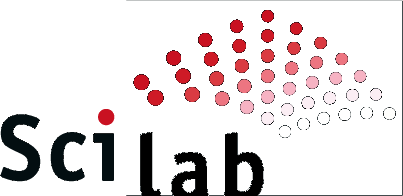
\includegraphics[height=.8cm]{png/logo_scilab}} 
\rotatebox{90}{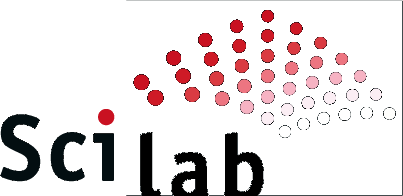
\includegraphics[height=.6cm]{png/logo_scilab}} 
        {\color{violetf}\vrule width 3pt}%
        \hspace{0pt}%must no space.
        \fboxsep=\FrameSep\colorbox{violetc}%
    }%
    \MakeFramed{\hsize #1 \advance\hsize-\width\FrameRestore}%
}%
{\endMakeFramed}%

\newenvironment{pseudo}[1][\hsize]%
{%
    \def\FrameCommand%
    {%
\rotatebox{90}{\textit{\textsf{Pseudo Code}}} 
        {\color{violetf}\vrule width 3pt}%
        \hspace{0pt}%must no space.
        \fboxsep=\FrameSep\colorbox{violetc}%
    }%
    \MakeFramed{\hsize #1 \advance\hsize-\width\FrameRestore}%
}%
{\endMakeFramed}%

\newenvironment{py}[1][\hsize]%
{%
    \def\FrameCommand%
    {%
%\rotatebox{90}{\textit{\textsf{Python}}} 
\rotatebox{90}{
\includegraphics[height=.6cm]{png/logo_python}} 
        {\color{violetf}\vrule width 3pt}%
        \hspace{0pt}%must no space.
        \fboxsep=\FrameSep\colorbox{violetc}%
    }%
    \MakeFramed{\hsize #1 \advance\hsize-\width\FrameRestore}%
}%
{\endMakeFramed}%


\newenvironment{term}[1][\hsize]%
{%
    \def\FrameCommand%
    {%
\rotatebox{90}{\textit{\textsf{Terminal}}} 
        {\color{violetf}\vrule width 3pt}%
        \hspace{0pt}%must no space.
        \fboxsep=\FrameSep\colorbox{violetc}%
    }%
    \MakeFramed{\hsize #1 \advance\hsize-\width\FrameRestore}%
}%
{\endMakeFramed}%



\newenvironment{comp}[1][\hsize]%
{%
    \def\FrameCommand
    {%
\rotatebox{90}{\textit{\textsf{Compétences}}} 
        {\color{bleuf}\vrule width 3pt}%
        \hspace{0pt}%must no space.
        \fboxsep=\FrameSep\colorbox{bleuc}%
    }%
    \MakeFramed{\hsize#1\advance\hsize-\width\FrameRestore}%
}%
{\endMakeFramed}%

\newenvironment{rem}[1][\hsize]%
{%
    \def\FrameCommand
    {%
\rotatebox{90}{\textit{\textsf{Remarque}}} 
        {\color{bleuf}\vrule width 3pt}%
        \hspace{0pt}%must no space.
        \fboxsep=\FrameSep\colorbox{bleuc}%
    }%
    \MakeFramed{\hsize#1\advance\hsize-\width\FrameRestore}%
}%
{\endMakeFramed}%


\newenvironment{savoir}[1][\hsize]%
{%
    \def\FrameCommand
    {%
\rotatebox{90}{\textit{\textsf{Savoir}}} 
        {\color{bleuf}\vrule width 3pt}%
        \hspace{0pt}%must no space.
        \fboxsep=\FrameSep\colorbox{bleuc}%
    }%
    \MakeFramed{\hsize#1\advance\hsize-\width\FrameRestore}%
}%
{\endMakeFramed}%

\newenvironment{Objectif}[1][\hsize]%
{%
    \def\FrameCommand
    {%
\rotatebox{90}{\textit{\textsf{Objectif}}} 
        {\color{bleuf}\vrule width 3pt}%
        \hspace{0pt}%must no space.
        \fboxsep=\FrameSep\colorbox{bleuc}%
    }%
    \MakeFramed{\hsize#1\advance\hsize-\width\FrameRestore}%
}%
{\endMakeFramed}%

\newenvironment{prob}[1][\hsize]%
{%
    \def\FrameCommand%
    {%
\rotatebox{90}{\textit{\textsf{ Problématique}}} 
        {\color{rougef}\vrule width 3pt}%
        \hspace{0pt}%must no space.
        \fboxsep=\FrameSep\colorbox{rougec}%
    }%
    \MakeFramed{\hsize#1\advance\hsize-\width\FrameRestore}%
}%
{\endMakeFramed}%

\newenvironment{obj}[1][\hsize]%
{%
    \def\FrameCommand%
    {%
\rotatebox{90}{\textit{\textsf{Objectifs}}} 
        {\color{rougef}\vrule width 3pt}%
        \hspace{0pt}%must no space.
        \fboxsep=\FrameSep\colorbox{rougec}%
    }%
    \MakeFramed{\hsize#1\advance\hsize-\width\FrameRestore}%
}%
{\endMakeFramed}%

\newenvironment{defi}[1][\hsize]%
{%
    \def\FrameCommand%
    {%
\rotatebox{90}{\textit{\textsf{Définition\\}}} 
        {\color{bleuf}\vrule width 3pt}%
        \hspace{0pt}%must no space.
        \fboxsep=\FrameSep\colorbox{bleuc}%
    }%
    \MakeFramed{\hsize#1\advance\hsize-\width\FrameRestore}%
}%
{\endMakeFramed}%


\newenvironment{demo}[1][\hsize]%
{%
    \def\FrameCommand%
    {%
\rotatebox{90}{\textit{\textsf{Démonstration\\}}} 
        {\color{bleuf}\vrule width 3pt}%
        \hspace{0pt}%must no space.
        \fboxsep=\FrameSep\colorbox{bleuc}%
    }%
    \MakeFramed{\hsize#1\advance\hsize-\width\FrameRestore}%
}%
{\endMakeFramed}%


\newenvironment{hypo}[1][\hsize]%
{%
    \def\FrameCommand%
    {%
\rotatebox{90}{\textit{\textsf{Hypothèse\\}}} 
        {\color{bleuf}\vrule width 3pt}%
        \hspace{0pt}%must no space.
        \fboxsep=\FrameSep\colorbox{bleuc}%
    }%
    \MakeFramed{\hsize#1\advance\hsize-\width\FrameRestore}%
}%
{\endMakeFramed}%


\newenvironment{prop}[1][\hsize]%
{%
    \def\FrameCommand%
    {%
\rotatebox{90}{\textit{\textsf{Propriété\\}}} 
        {\color{bleuf}\vrule width 3pt}%
        \hspace{0pt}%must no space.
        \fboxsep=\FrameSep\colorbox{bleuc}%
    }%
    \MakeFramed{\hsize#1\advance\hsize-\width\FrameRestore}%
}%
{\endMakeFramed}%

\newenvironment{props}[1][\hsize]%
{%
    \def\FrameCommand%
    {%
\rotatebox{90}{\textit{\textsf{Propriétés\\}}} 
        {\color{bleuf}\vrule width 3pt}%
        \hspace{0pt}%must no space.
        \fboxsep=\FrameSep\colorbox{bleuc}%
    }%
    \MakeFramed{\hsize#1\advance\hsize-\width\FrameRestore}%
}%
{\endMakeFramed}%

\newenvironment{exemple}[1][\hsize]%
{%
    \def\FrameCommand%
    {%
\rotatebox{90}{\textit{\textsf{Exemple\\}}} 
        {\color{vertf}\vrule width 3pt}%
        \hspace{0pt}%must no space.
        \fboxsep=\FrameSep\colorbox{vertc}%
    }%
    \MakeFramed{\hsize#1\advance\hsize-\width\FrameRestore}%
}%
{\endMakeFramed}%

\newenvironment{exercice}[1][\hsize]%
{%
    \def\FrameCommand%
    {%
\rotatebox{90}{\textit{\textsf{Exercice\\}}} 
        {\color{vertf}\vrule width 3pt}%
        \hspace{0pt}%must no space.
        \fboxsep=\FrameSep\colorbox{vertc}%
    }%
    \MakeFramed{\hsize#1\advance\hsize-\width\FrameRestore}%
}%
{\endMakeFramed}%

\newenvironment{Support}[1][\hsize]%
{%
    \def\FrameCommand%
    {%
\rotatebox{90}{\textit{\textsf{Support de cours\\}}} 
        {\color{vertf}\vrule width 3pt}%
        \hspace{0pt}%must no space.
        \fboxsep=\FrameSep\colorbox{jaunec}%
    }%
    \MakeFramed{\hsize#1\advance\hsize-\width\FrameRestore}%
}%
{\endMakeFramed}%

\newenvironment{resultat}[1][\hsize]%
{%
    \def\FrameCommand%
    {%
\rotatebox{90}{\textit{\textsf{Résultat\\}}} 
        {\color{rougef}\vrule width 3pt}%
        \hspace{0pt}%must no space.
        \fboxsep=\FrameSep\colorbox{rougec}%
    }%
    \MakeFramed{\hsize#1\advance\hsize-\width\FrameRestore}%
}%
{\endMakeFramed}%

\newenvironment{methode}[1][\hsize]%
{%
    \def\FrameCommand%
    {%
\rotatebox{90}{\textit{\textsf{Méthode\\}}} 
        {\color{rougef}\vrule width 3pt}%
        \hspace{0pt}%must no space.
        \fboxsep=\FrameSep\colorbox{rougec}%
    }%
    \MakeFramed{\hsize#1\advance\hsize-\width\FrameRestore}%
}%
{\endMakeFramed}%

\newenvironment{theo}[1][\hsize]%
{%
    \def\FrameCommand%
    {%
\rotatebox{90}{\textit{\textsf{Théorème\\}}} 
        {\color{rougef}\vrule width 3pt}%
        \hspace{0pt}%must no space.
        \fboxsep=\FrameSep\colorbox{rougec}%
    }%
    \MakeFramed{\hsize#1\advance\hsize-\width\FrameRestore}%
}%
{\endMakeFramed}%

\newenvironment{warn}[1][\hsize]%
{%
    \def\FrameCommand%
    {%
\rotatebox{90}{\textit{\textsf{Attention\\}}} 
        {\color{rougef}\vrule width 3pt}%
        \hspace{0pt}%must no space.
        \fboxsep=\FrameSep\colorbox{rougec}%
    }%
    \MakeFramed{\hsize#1\advance\hsize-\width\FrameRestore}%
}%
{\endMakeFramed}%

%Si le boolen xp est vrai : compilation pour xabi
%Sinon compilation Damien
\newboolean{xp}
\setboolean{xp}{true}

\newboolean{prof}
\setboolean{prof}{true}

\usepackage[%
    pdftitle={CI 06 : Stat - Modélisation des AM},
    pdfauthor={Xavier Pessoles},
    colorlinks=true,
    linkcolor=blue,
    citecolor=magenta]{hyperref}


\def\discipline{Sciences Industrielles de l'Ingénieur}
\def\xxtitre{\ifthenelse{\boolean{xp}}{
CI 06 : Étude du comportement statique des systèmes}{}}

\def\xxsoustitre{\ifthenelse{\boolean{xp}}{
Chapitre 1 -- Modélisation des Actions Mécaniques}{
Partie  -- }}

\def\xxauteur{\ifthenelse{\boolean{xp}}{
Xavier \textsc{Pessoles}}{}}

\def\xxpied{\ifthenelse{\boolean{xp}}{
CI 06 : Statique\\
Ch. 1 : Modélisation des AM -- Cours}{
\xxtitre}}

\def\xxcathegorie{\ifthenelse{\boolean{xp}}{
2013 -- 2014 \\
Xavier \textsc{Pessoles}}{}}





%---------------------------------------------------------------------------


\begin{document}

\ifthenelse{\boolean{xp}}{
\sloppy
\hyphenpenalty 10000


%------------- En tetes et Pieds de Pages ------------

\pagestyle{fancy}
\renewcommand{\headrulewidth}{0pt}
\fancyhead{}
\fancyhead[L]{%
\noindent\begin{minipage}[c]{2.6cm}%
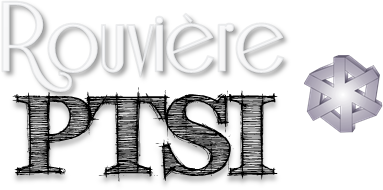
\includegraphics[width=2cm]{png/logo_ptsi.png}%
\end{minipage}}


\fancyhead[C]{\rule{12cm}{.5pt}}


\fancyhead[R]{%
\noindent\begin{minipage}[c]{3cm}
\begin{flushright}
\footnotesize{\textit{\textsf{\discipline}}}%
\end{flushright}
\end{minipage}
}



\fancyhead[C]{\rule{12cm}{.5pt}}

\renewcommand{\footrulewidth}{0.2pt}

\fancyfoot[C]{\footnotesize{\bfseries \thepage}}
\fancyfoot[L]{%
\begin{minipage}[c]{.4\linewidth}
\noindent\footnotesize{{\xxauteur}}
\end{minipage}
}

\fancyfoot[R]{\footnotesize{\xxpied}}

\begin{center}
 \iftd
 \Large\textsc{\xxtitre}
 \else
 \huge\textsc{\xxtitre}
 \fi
\end{center}

\begin{center}
 \iftd
 \large\textsc{\xxsoustitre}
 \else
 \LARGE\textsc{\xxsoustitre}
 \fi
\end{center}

\vspace{.5cm}
}{\ifthenelse{\boolean{xp}}{
\usepackage[%
    pdftitle={OS et Environnement de développement},
    pdfauthor={Xavier Pessoles},
    colorlinks=true,
    linkcolor=blue,
    citecolor=magenta]{hyperref}}{
\usepackage[%
    pdftitle={OS et Environnement de développement},
    pdfauthor={Damien Iceta},
    colorlinks=true,
    linkcolor=blue,
    citecolor=magenta]{hyperref}}

\usepackage{pifont}
\usepackage{lastpage}

% \makeatletter \let\ps@plain\ps@empty \makeatother
%% DEBUT DU DOCUMENT
%% =================
\sloppy
\hyphenpenalty 10000

\newcommand{\Pointilles}[1][3]{%
\multido{}{#1}{\makebox[\linewidth]{\dotfill}\\[\parskip]
}}


\colorlet{shadecolor}{orange!15}

\newtheorem{theorem}{Theorem}


\begin{document}


\newboolean{prof}
\setboolean{prof}{true}
%------------- En tetes et Pieds de Pages ------------


\pagestyle{fancy}
%\renewcommand{\headrulewidth}{0}
\renewcommand{\headrulewidth}{0.2pt} %pour mettre le trait en haut

\fancyhead{}
\fancyhead[L]{
\footnotesize{{{\xxtitre}}}%
%\noindent\noindent\begin{minipage}[c]{2.6cm}
%\includegraphics[width=2.5cm]{png/logo.png}%
%\end{minipage}
}

%\fancyhead[C]{\rule{12cm}{.5pt}}  %pour mettre le petit trait en haut


\fancyhead[R]{%
\noindent\begin{minipage}[c]{3cm}
\begin{flushright}
\footnotesize{{{\xxcathegorie}}}%
\end{flushright}
\end{minipage}
}

\renewcommand{\footrulewidth}{0.2pt}

\fancyfoot[C]{\footnotesize{}}
\fancyfoot[L]{%
\begin{minipage}[l]{.2\linewidth}
\noindent\footnotesize{{\xxauteur}}
\end{minipage}
\begin{minipage}[c]{.15\linewidth}
%
\includegraphics[width=2cm]{png/logoCC.png}
\end{minipage}}

\ifthenelse{\boolean{prof}}{%
\fancyfoot[R]{\footnotesize{Page \thepage\   sur  \pageref{LastPage}}}}

\begin{center}
 \huge\textsc{\xxtitre}
\end{center}

\begin{center}
 \LARGE\textsc{\xxsoustitre}
\end{center}

\vspace{.5cm}}



\vspace{.5cm}

\begin{center}
\begin{tabular}{ccc}
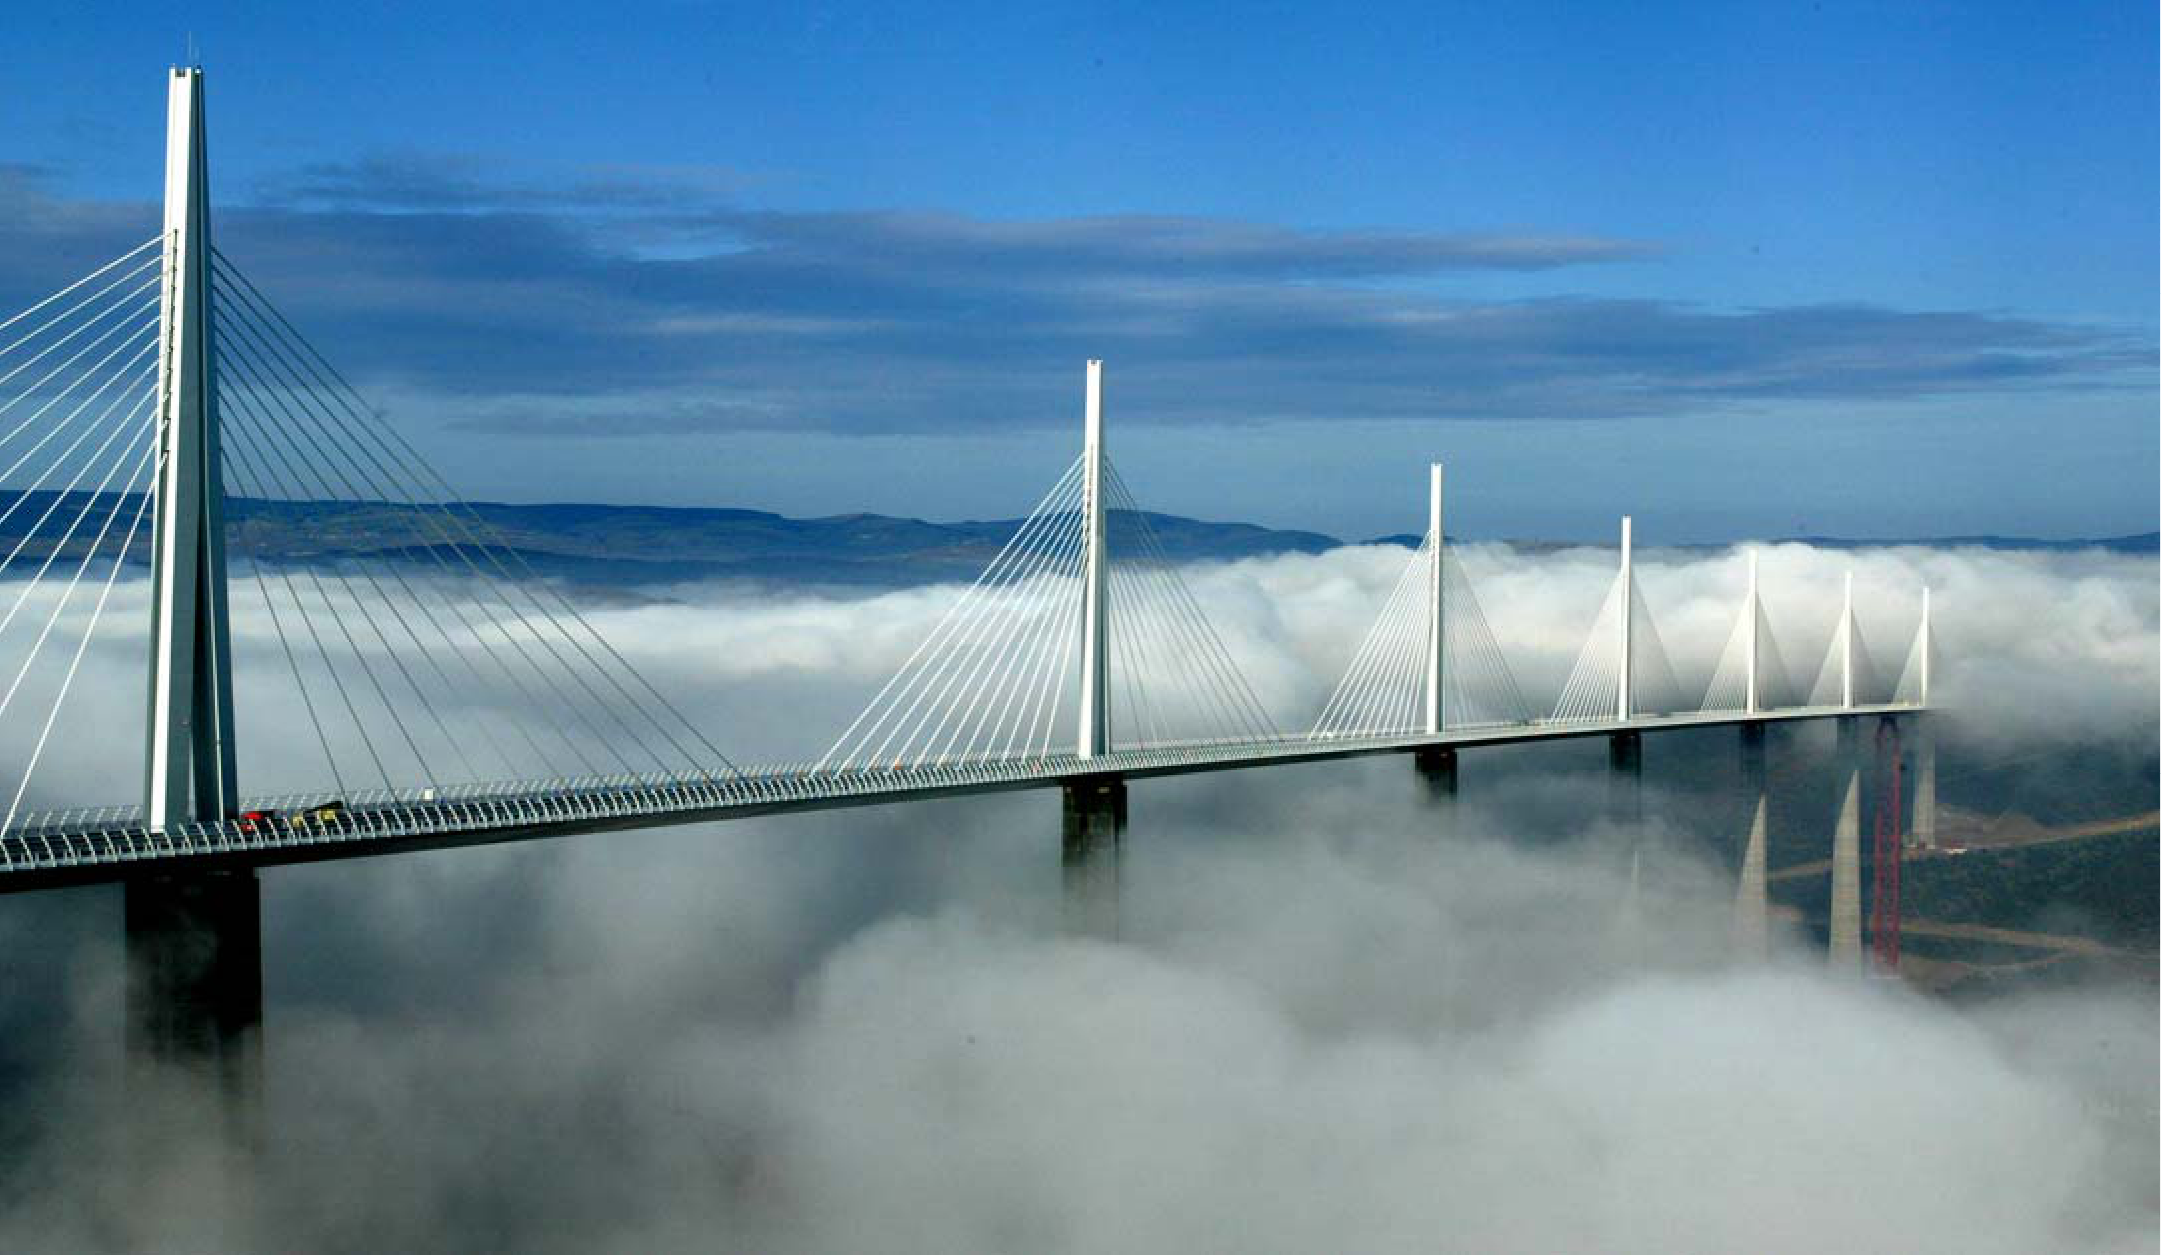
\includegraphics[height=3cm]{images/millau} &
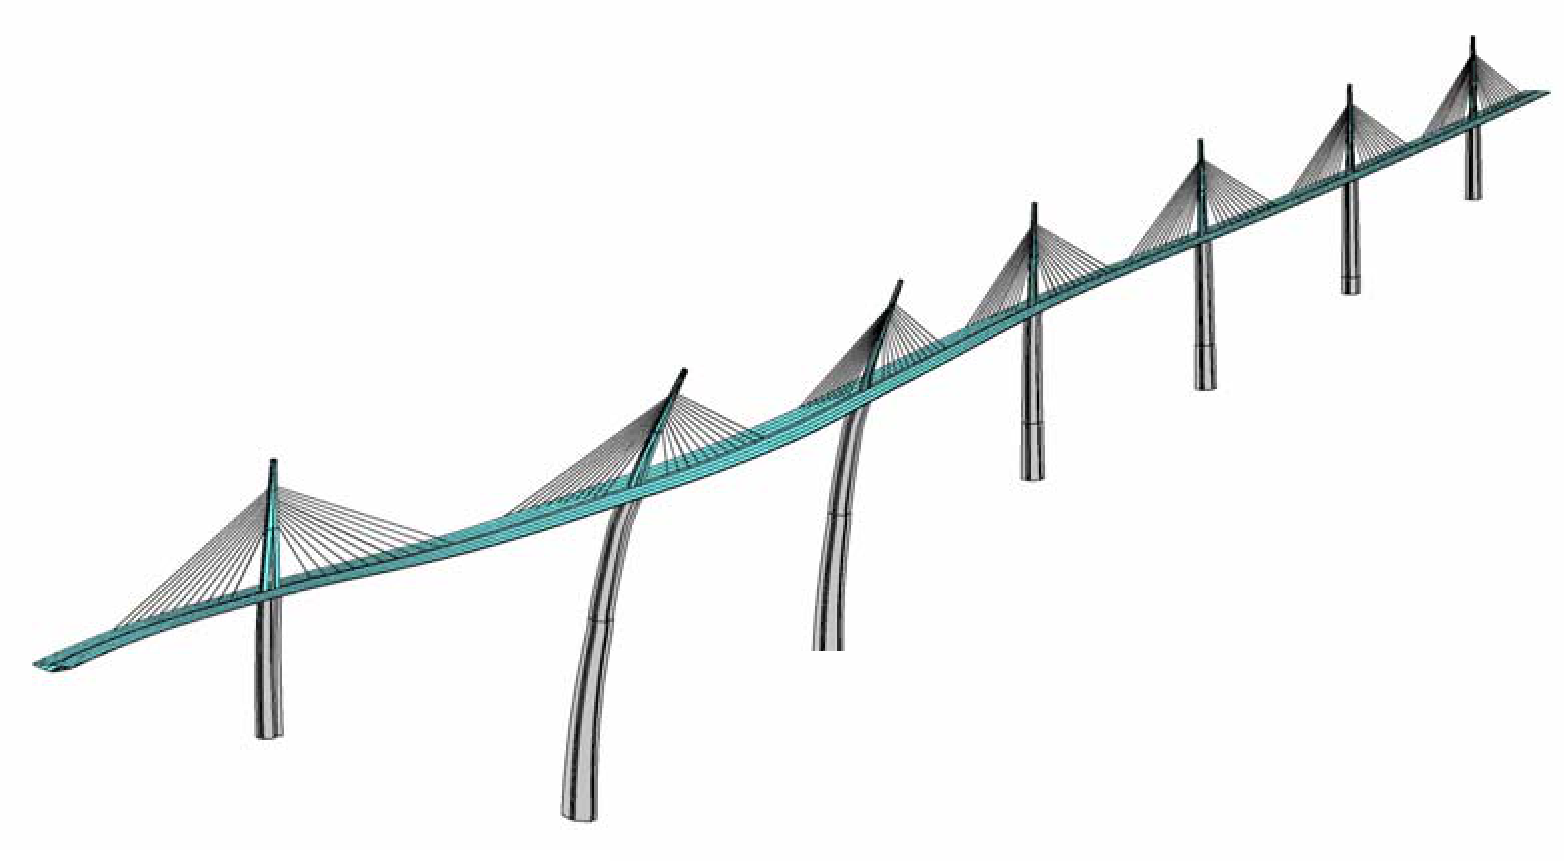
\includegraphics[height=3cm]{images/millau2} &
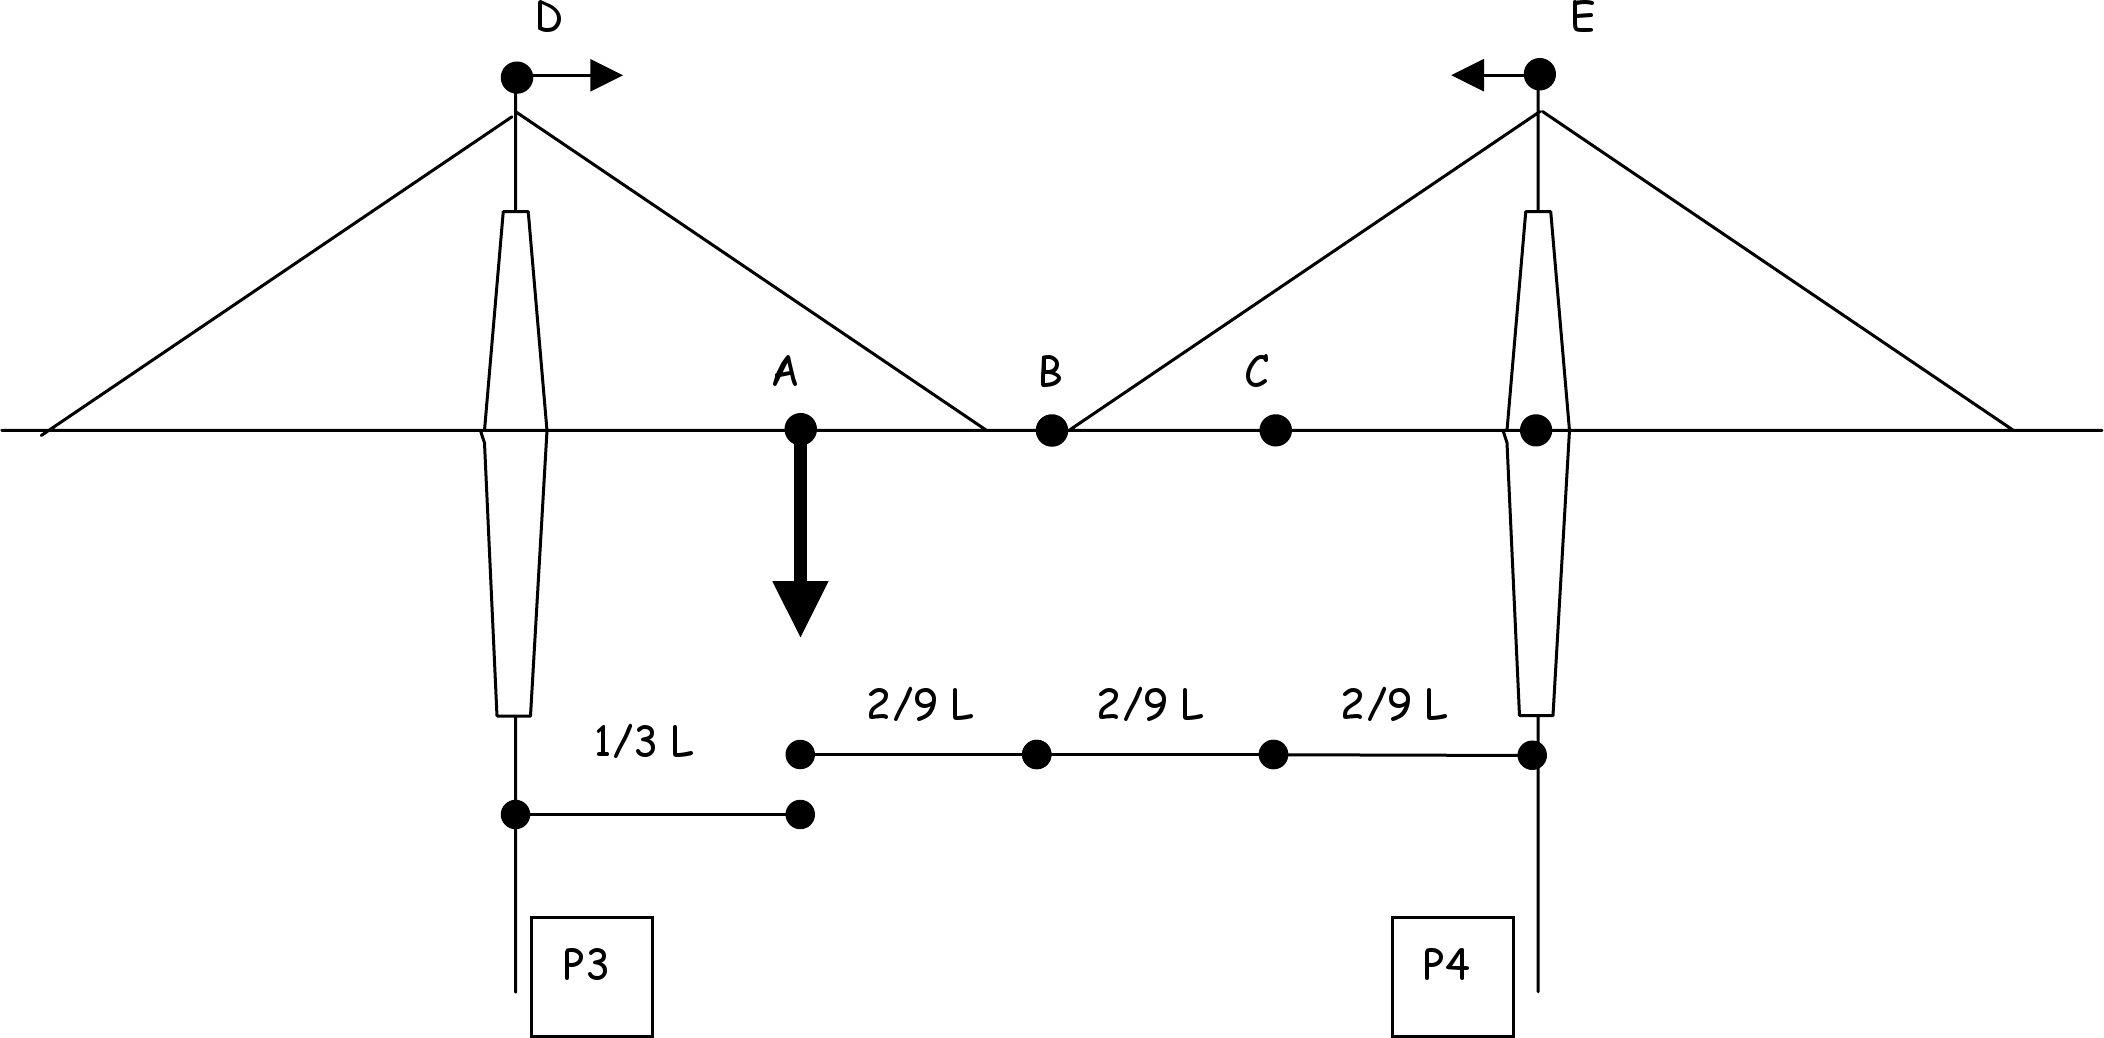
\includegraphics[height=3cm]{images/millau3} \\
\textit{Viaduc de Millau \cite{millau1}} & \textit{Mode de flexion \cite{millau1}}&\textit{Sollicitation de la structure \cite{millau1}}\\
\end{tabular}
\end{center}

Le dimensionnement des structures mécaniques passe par la connaissance des efforts qui vont s'appliquer à elle. Le viaduc de Millau doit par exemple supporter les efforts dus au passage des différents véhicules (moto, voiture, bus, camions, ...) à l'effort du vent. Ces efforts sont supportés d'une part par les piles du pont et d'autre part par les différents haubans. Ceux-ci doivent aussi être dimensionnés pour supporter le poids du tablier et le poids des piles elle-mêmes.

Ainsi, la connaissance des efforts s'exerçant sur la structure permettra de les dimensionner afin de résister aux différentes sollicitations.

\vspace{.2cm}

\begin{prob}
\textsc{Problématique :}
\begin{itemize}
\item Comment modéliser un système afin de réaliser une étude de statique ?
\item Comment modéliser les efforts s'exerçant sur système ?
\end{itemize}
\end{prob}

\begin{savoir}
\textsc{Savoirs :}
\begin{itemize}
\item Mod-C15 : Modélisation des actions mécaniques
\begin{itemize}
\item Mod-C15.1 : Modèle local (densité surfacique, linéique et volumique d’effort) :
\begin{itemize}
\item contact parfait ;
\item modélisation du frottement sec -- Lois de Coulomb ;
%\item modélisation de résistance au roulement ;
%\item modélisation de résistance au pivotement.
\end{itemize}
\item Mod-C15.2 : Modèle global (torseur d’action mécanique)
\item Mod-C15.3 : Modèle global du frottement visqueux.
\end{itemize}
\begin{itemize}
\item Mod-C15-S1 : Associer un modèle à une action mécanique.
\item Mod-C15-S2 : Écrire la relation entre le modèle local et le modèle global associé aux actions mécaniques dans les cas suivants : action d’un fluide, action entre solides (liaisons avec et sans frottement).
\item Mod-C15-S3 : Écrire le modèle global de l’action de la pesanteur, du frottement fluide, de la résistance au roulement et du pivotement.
\item Mod-C15-S4 : Associer un modèle global d’effort au comportement d’une liaison réelle.
\end{itemize}
\end{itemize}
\end{savoir}

\setlength{\parskip}{0ex plus 0.2ex minus 0ex}
 \renewcommand{\contentsname}{}
 \renewcommand{\baselinestretch}{1}

\tableofcontents

 \renewcommand{\baselinestretch}{1.2}
\setlength{\parskip}{2ex plus 0.5ex minus 0.2ex}

% \vspace{1cm}
\textit{Ce document est en évolution permanente. Merci de signaler toutes
erreurs ou coquilles.}

\section{Définitions}

\begin{hypo}
En statique, les solides (ou systèmes matériels) étudiés sont supposés :
\begin{itemize}
\item géométriquement parfaits;
\item indéformables; 
\item de masse constante. 
\end{itemize}
\end{hypo}


\begin{defi}
\textbf{Systèmes matériels}

Quantité de matière dont la masse reste constante pendant l'étude. On note $S$ un système matériel et $\overline{S}$ l'extérieur de $S$.
\end{defi}

\begin{rem}
Un système matériel peut être un solide, un ensemble de solides, une partie de solide, un fluide.
\end{rem}

\begin{exemple}
\textit{Vérin double effet Festo \cite{verin}}

\begin{minipage}[c]{.3\linewidth}
\begin{center}
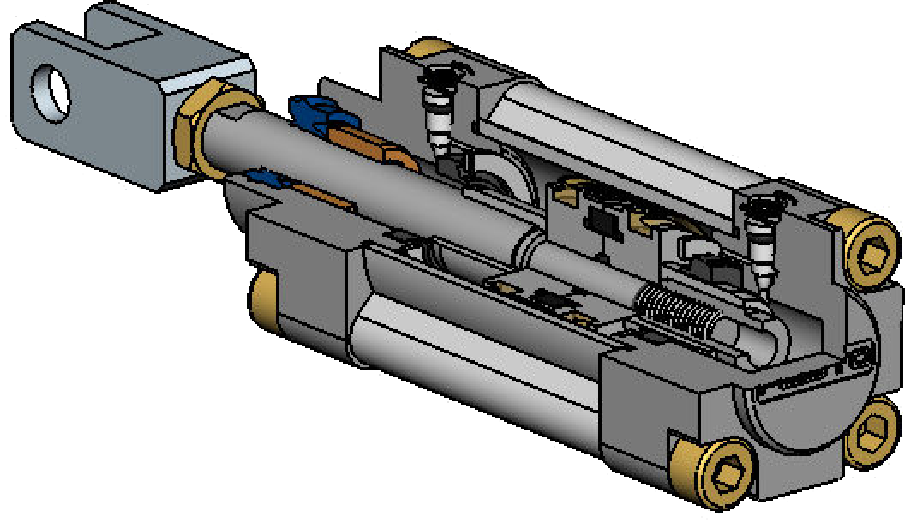
\includegraphics[width=\textwidth]{images/verin2}
\end{center}
\end{minipage}\hfill
\begin{minipage}[c]{.6\linewidth}
\begin{center}
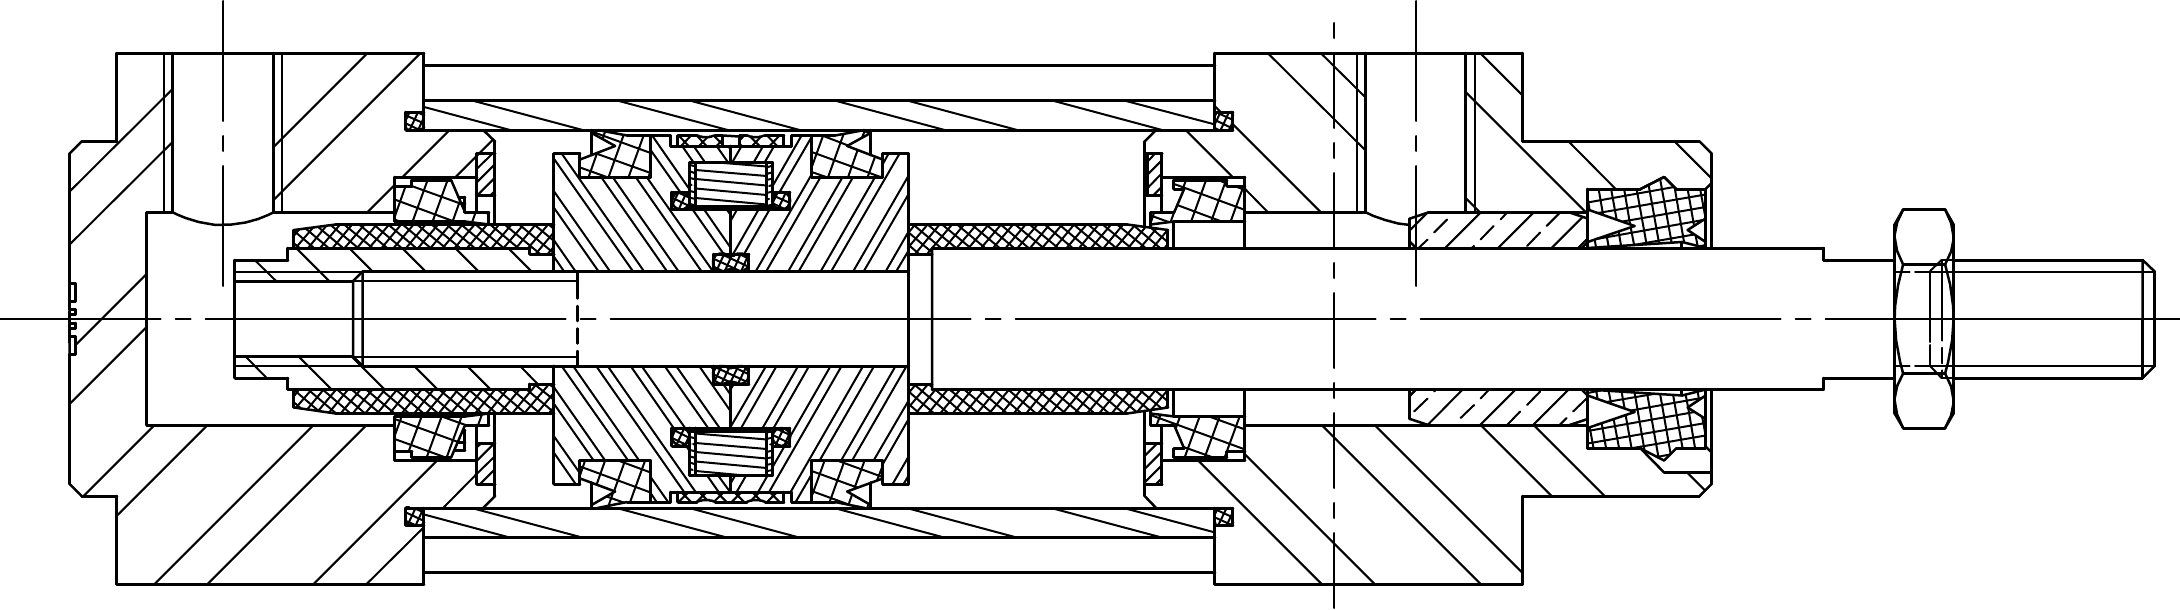
\includegraphics[width=\textwidth]{images/verin1}
\end{center}
\end{minipage}

La tige de vérin peut être considérée comme un solide. Le piston, avec toutes les pièces qui le composent, peut être considéré comme un système matériel. 

Le fluide peut aussi être considéré comme un ensemble matériel. 
\end{exemple}


%\begin{defi}
%\end{defi}


\subsection{Action mécanique}
\begin{defi}
\textbf{Action mécanique (AM)}

Une action mécanique désigne tout phénomène physique capable de provoquer un mouvement ou une déformation d'un système matériel.
\end{defi}

\begin{exemple}

\begin{minipage}[c]{.47\linewidth}
\begin{center}
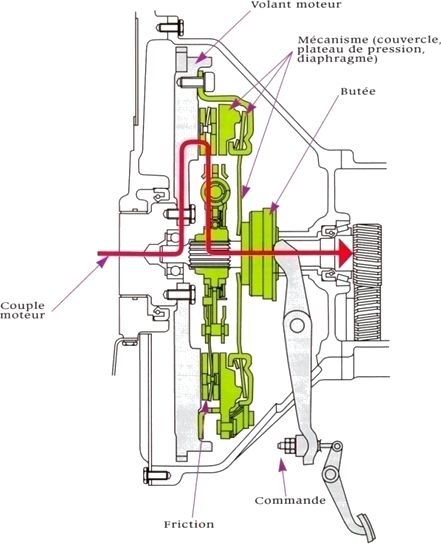
\includegraphics[width=.7\textwidth]{images/embrayage}

\textit{Embrayage de voiture}
\end{center}

\end{minipage}\hfill
\begin{minipage}[c]{.47\linewidth}
\begin{center}
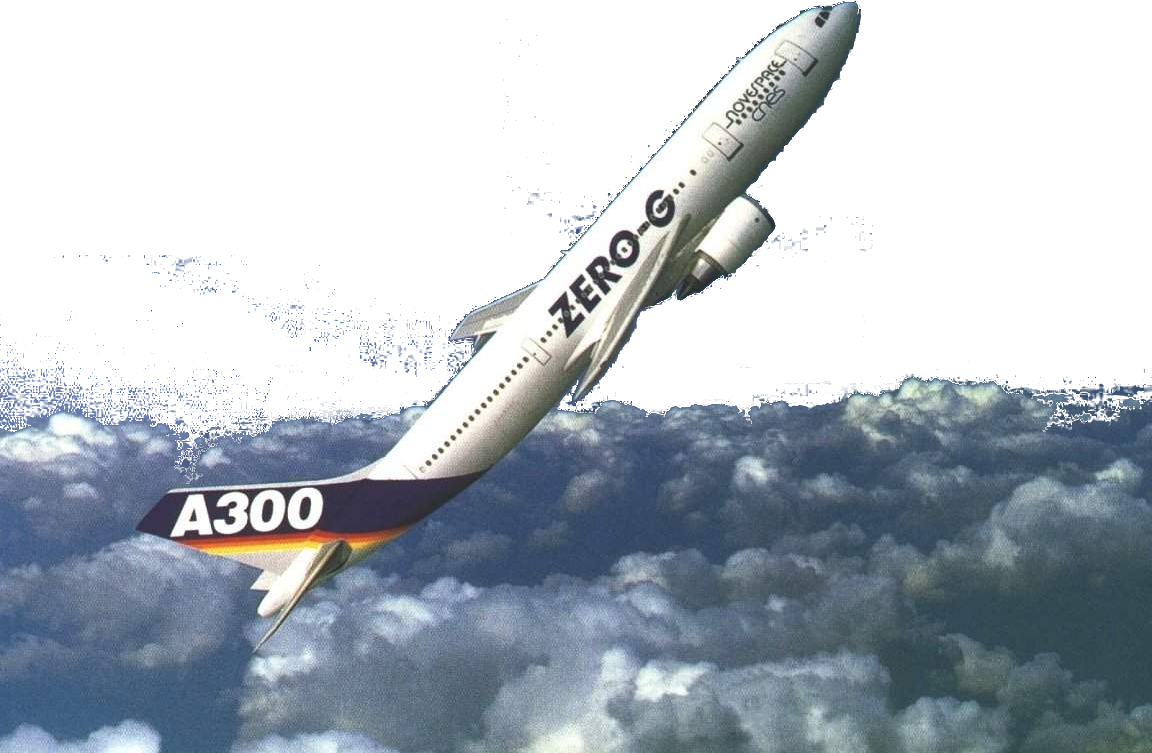
\includegraphics[width=.7\textwidth]{images/zerog}

\textit{Airbus Zéro G \cite{zerog}}
\end{center}
\end{minipage}

On distingue :
\begin{itemize}
\item les actions mécaniques de contact : elles s'appliquent sur la surface (ou une portion de surface) d'un système matériel (action d'un système matériel sur un autre, action d'un fluide sur un système matériel);
\item les actions mécaniques à distance : elles s'appliquent sur tout le volume d'un système matériel (pesanteur, actions magnétiques).
\end{itemize}

\end{exemple}


Suivant le point de vue utilisé, les actions mécaniques peuvent être modélisées par : 
\begin{itemize}
\item le modèle local, qui s'intéresse aux actions en chaque point de la surface de contact entre deux systèmes matériels (ou en tout point du volume s'il s'agit d'actions volumiques);
\item le modèle global, qui, à partir de la modélisation locale, permet de se ramener à une action en un point. 
\end{itemize}

\begin{center}
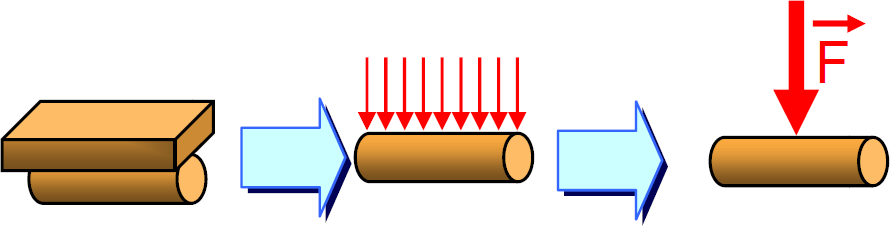
\includegraphics[width=.5\textwidth]{images/local_global}
\end{center}

\begin{defi}
\begin{minipage}[c]{.65\linewidth}
\textbf{Force élémentaire}

Une force élémentaire $d\vect{R_{\text{ext}\rightarrow S}}$ est une action mécanique extérieure ($ext$) s'exerçant sur une partie d'un système matériel $S$:
\begin{itemize}
\item un élément linéique $dl$ ($m$);
\item un élément surfacique $dS$ ($m^2$);
\item un élément de volumique $d\mathcal{V}$ ($m^3$).
\end{itemize} 
Cette force est représentable par un glisseur $(M,d\vect{R_{(\text{ext}\rightarrow S)}})$ où $M$ est le point d'application. On note $\vect{u(M)}$ la direction de l'effort. $||d\vect{R_{(\text{ext}\rightarrow S)}}||$ s'exprime en Newton (N).

On note $f(M)$ la fonction densité d'effort. Suivant que l'action mécanique s'exerce sur une ligne, une surface ou un volume, on parlera de densité d'effort linéique (en $N/m$), surfacique (en $N/m^2$) ou volumique (en $N/m^3$).

On a donc :
$$
d\vect{R_{(\text{ext}\rightarrow S)}} = f(M) \vect{u(M)} dV 
$$

Respectivement, $d\vect{R_{(\text{ext}\rightarrow S)}} = f(M) \vect{u(M)} dl $ et $d\vect{R_{(\text{ext}\rightarrow S)}} = f(M) \vect{u(M)} dS $ en respectant l'homogénéité de la force.
\end{minipage}\hfill
\begin{minipage}[c]{.3\linewidth}
\begin{center}
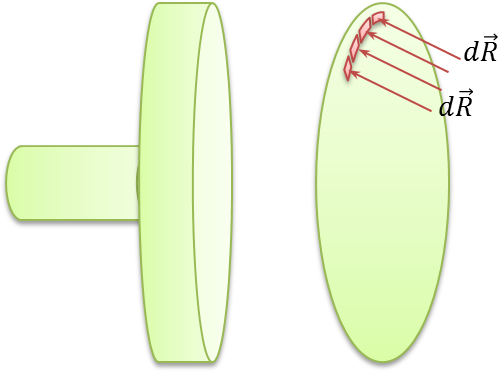
\includegraphics[width=.95\textwidth]{images/local}
\end{center}
\end{minipage}
\end{defi}

\begin{defi}
\begin{minipage}[c]{.65\linewidth}
\textbf{Force globale}

La force globale extérieure agissant sur un système matériel $S$ se calcule alors ainsi : 
$$
\vect{R_{(\text{ext}\rightarrow S)}} 
= \iiint\limits_{\mathcal{V}} d\vect{R_{(\text{ext}\rightarrow S)}} 
= \iiint\limits_{\mathcal{V}} f(M) \vect{u(M)} d\mathcal{V}
$$
\end{minipage} \hfill
\begin{minipage}[c]{.3\linewidth}
\begin{center}
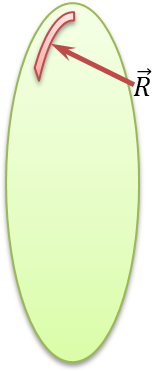
\includegraphics[width=.5\textwidth]{images/global}
\end{center}
\end{minipage}
\end{defi}

\begin{exemple}
\begin{minipage}[c]{.3\linewidth}
\begin{center}
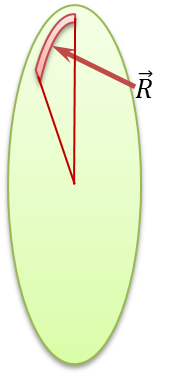
\includegraphics[width=.5\textwidth]{images/result_couronne}
\end{center}
\end{minipage}
\hfill
\begin{minipage}[c]{.65\linewidth}
Une portion de couronne est soumise à une pression uniforme $p$. Les dimensions de la surface sont les suivantes : 
\begin{itemize}
\item $r$ : << petit >> rayon;
\item $R$ : << grand >> rayon;
\item $\alpha$ : portion angulaire.
\end{itemize}
Calculer l'effort résultant. 
\end{minipage}

Un demi cylindre de rayon $r$ et de longueur $h$ est soumis à un champ de pression uniforme $p$ orienté suivant la normale au cylindre. 
\begin{enumerate}
\item Déterminer la résultante des efforts. 
\item Qu'en est-il si le champ de pression est de la forme $p_0 \cos \theta$ ?
\end{enumerate}


\end{exemple}

\begin{defi}
\textbf{Moment d'une force}

Soit une force élémentaire appliquée au point $M$ : $d\vectf{\text{ext}}{S}$. On appelle moment élémentaire de la force $d\vectf{\text{ext}}{S}$ au point $P$ le vecteur défini par : 
$$
d\vectm{P}{\text{ext}}{S} = \vect{PM}\wedge d\vectf{\text{ext}}{S}
$$

Par intégration, le moment global s'exprime donc ainsi : 
$$
\vectm{P}{\text{ext}}{S} = \iiint\limits_{\mathcal{V}}d\vectm{P}{\text{ext}}{S} 
$$


\end{defi}




\begin{rem}
\textit{Moment d'une force -- Interprétation graphique}

Prenons le cas du serrage d'un écrou avec un effort $\vect{F}=-F\vect{y}$ :

\begin{center}
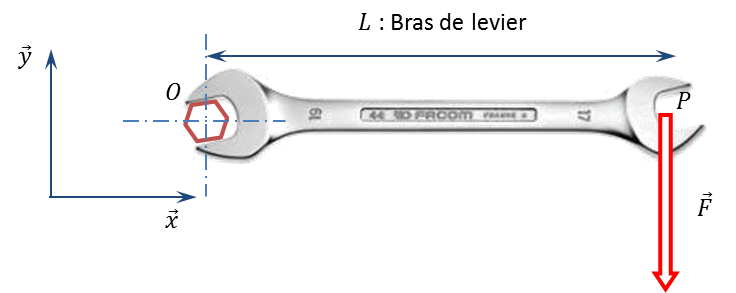
\includegraphics[width=.6\textwidth]{images/clef}
\end{center}

Dans l'hypothèse où l'effort $\vect{F}$ s'appliquerait au point $O$, il n'y aurait donc pas de serrage de l'écrou. Le moment (ou couple de serrage) serait donc nul : $\vectm{O}{\text{Clef}}{\text{Ecrou}}=\vect{0}$.

Si l'effort s'applique en $P$, 
$$\vectm{O}{\text{Clef}}{\text{Ecrou}}=\vect{OP}\wedge\vect{F}
=L\vect{x}\wedge-F\vect{y}=-LF\vect{z}$$

Pour un même effort, la norme du moment augmente quand le bras de levier augmente.

\end{rem}


\begin{exemple}
\begin{minipage}[c]{.3\linewidth}
\begin{center}
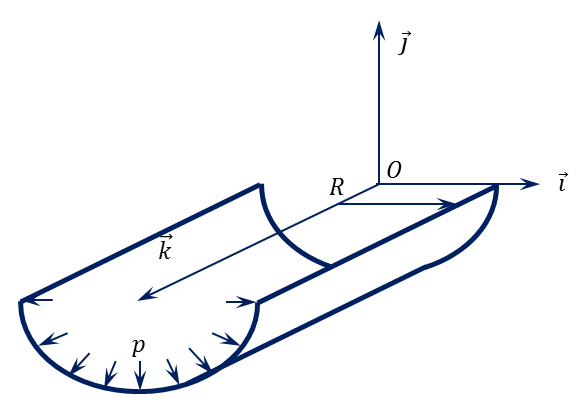
\includegraphics[width=\textwidth]{images/cyl_p}
\end{center}
\end{minipage}
\hfill
\begin{minipage}[c]{.65\linewidth}
Un demi cylindre de rayon $R$ et de longueur $h$ est soumis à un champ de pression uniforme $p$ orienté suivant la normale au cylindre. 

\begin{enumerate}
\item Déterminer la moment résultant du champ de pression.  
\item Qu'en est-il si le champ de pression est de la forme $p_0 \cos \theta$ ?
\end{enumerate}


\end{minipage}

\end{exemple}

\subsection{Torseur statique}

\begin{defi}
\textbf{Torseur statique ou torseur sthénique ou torseur d'efforts}

L'action mécanique d'un système matériel $S_1$ (ou d'un phénomène physique) sur un système matériel $S_2$ est représentable par un torseur au point M:
$$
\torseurstat{T}{S_2}{S_1}=
\torseurl{%
\vect{R_{(S_2\rightarrow S_1)}} 
= \iiint\limits_{\mathcal{V}} f(M) \vect{u(M)} d\mathcal{V}}{%
\vectm{P}{S_2}{S_1} = \iiint\limits_{\mathcal{V}}\vect{PM}\wedge d\vectf{S_2}{S_1}}{P}
$$

Il est aussi possible d'écrire ce torseur en colonne : 
$$
\torseurstat{T}{S_2}{S_1}
=\torseurl{\vectf{S_2}{S_1}}{\vectm{M}{S_2}{S_1}}{M}
=\torseurcol{X_{12}}{Y_{12}}{Z_{12}}{L_{12}}{M_{12}}{N_{12}}{M,\mathcal{R}}
$$
\end{defi}
\begin{rem}
La norme de vecteur $\vectf{S_2}{S_1}$ est en Newton (N). La norme du vecteur $\vectm{M}{S_2}{S_1}$ est en Newton -- mètre ($N\cdot m$).
\end{rem}

\begin{prop}
Le torseur statique étant un torseur, on a donc : 

$$
\forall B, \vectm{B}{S_2}{S_1} = \vectm{A}{S_2}{S_1} + \vect{BA} \wedge \vectf{S_2}{S_1}
$$
\end{prop}

\section{Actions mécaniques à distance}
\subsection{Action mécanique de pesanteur}

\begin{defi}
\textbf{Masse d'un solide}

Soit un solide de masse volumique $\mu$ et de volume $\mathcal{V}$. Sa masse $m$ est définie par : 
$$
m=\int\limits_{\mathcal{V}}\mu d\mathcal{V}
$$

\end{defi}

\begin{defi}
\textbf{Centre d'inertie d'un solide -- Programme PT}

Soit un point $M$ quelconque et un solide $S$ de masse $m$. Soit $P$ un point appartenant à $S$. Le centre d'inertie (ou centre de gravité ou centre de masse) est le point $G$ défini par : 
$$
\vect{MG}=\dfrac{1}{m} \int\vect{MP} dm
$$

\end{defi}


\begin{defi}
\textbf{Centre d'inertie d'un système matériel}

Soient un système matériel $E$ de masse $m$, composé de $n$ solides $S_i$ de masse $m_i$ et de centre d'inertie $G_i$. Le centre d'inertie d'inertie $G$ de $E$ est défini par : 
$$
\vect{MG} =\dfrac{1}{m}\sum\limits_{i=1}^{n} m_i \vect{MG_i}
$$

\end{defi}

\begin{defi}
\textbf{Action mécanique de pesanteur ou gravité}

Soit un solide $S$ situé dans un champ de pesanteur uniforme $\vect{g}$ et de volume $\mathcal{V}$. 

On note $G$ son centre de gravité. 

Le vecteur densité de force est donné par : $f(M)\vect{u(M)} = \mu(M) \vect{g}$ où $\mu(M)$ désigne la masse volumique du solide (en $kg/m^3$). 

Au \textbf{centre d'inertie} du système $G$, on peut exprimer le torseur des actions mécaniques :
$$
\torseurstat{T}{\text{Pesanteur}}{S} =
\torseurl{%
\vectf{\text{Pesanteur}}{S}=\iiint\limits_{\mathcal{V}}\mu(M)\vect{g}d\mathcal{V}}{%
\vectm{G}{\text{Pesanteur}}{S}=\vect{0}}{%
G}
=
\torseurl{%
\vectf{\text{Pesanteur}}{S}=m\vect{g}}{%
\vectm{G}{\text{Pesanteur}}{S}=\vect{0}}{%
G}
$$

\end{defi}

\begin{rem}
$\vect{g}$ est le champ de pesanteur terrestre, supposé uniforme à la surface de la terre. Dans la réalité il dépend de la latitude et de l'altitude. Il est orienté vers le centre de la terre et définit la verticale. 

Dans la pratique, on prendra $||\vect{g}||=9,81 \; m/s^2$.
\end{rem}
%
%\begin{exemple}
%\textit{Calcul de masse d'un tore de petit rayon $r$ et de grand rayon $R$ et de masse volumique $\mu$ (en $kg/m^3$)}
%
%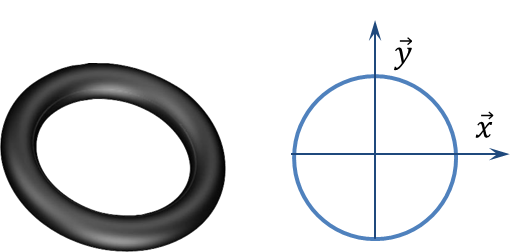
\includegraphics[width=.35\textwidth]{images/tore1}
%
%\vspace{6cm}
%\end{exemple}

\begin{exemple}
\textit{Calcul de masse d'une sphère de masse volumique $\mu$ (en $kg/m^3$).}

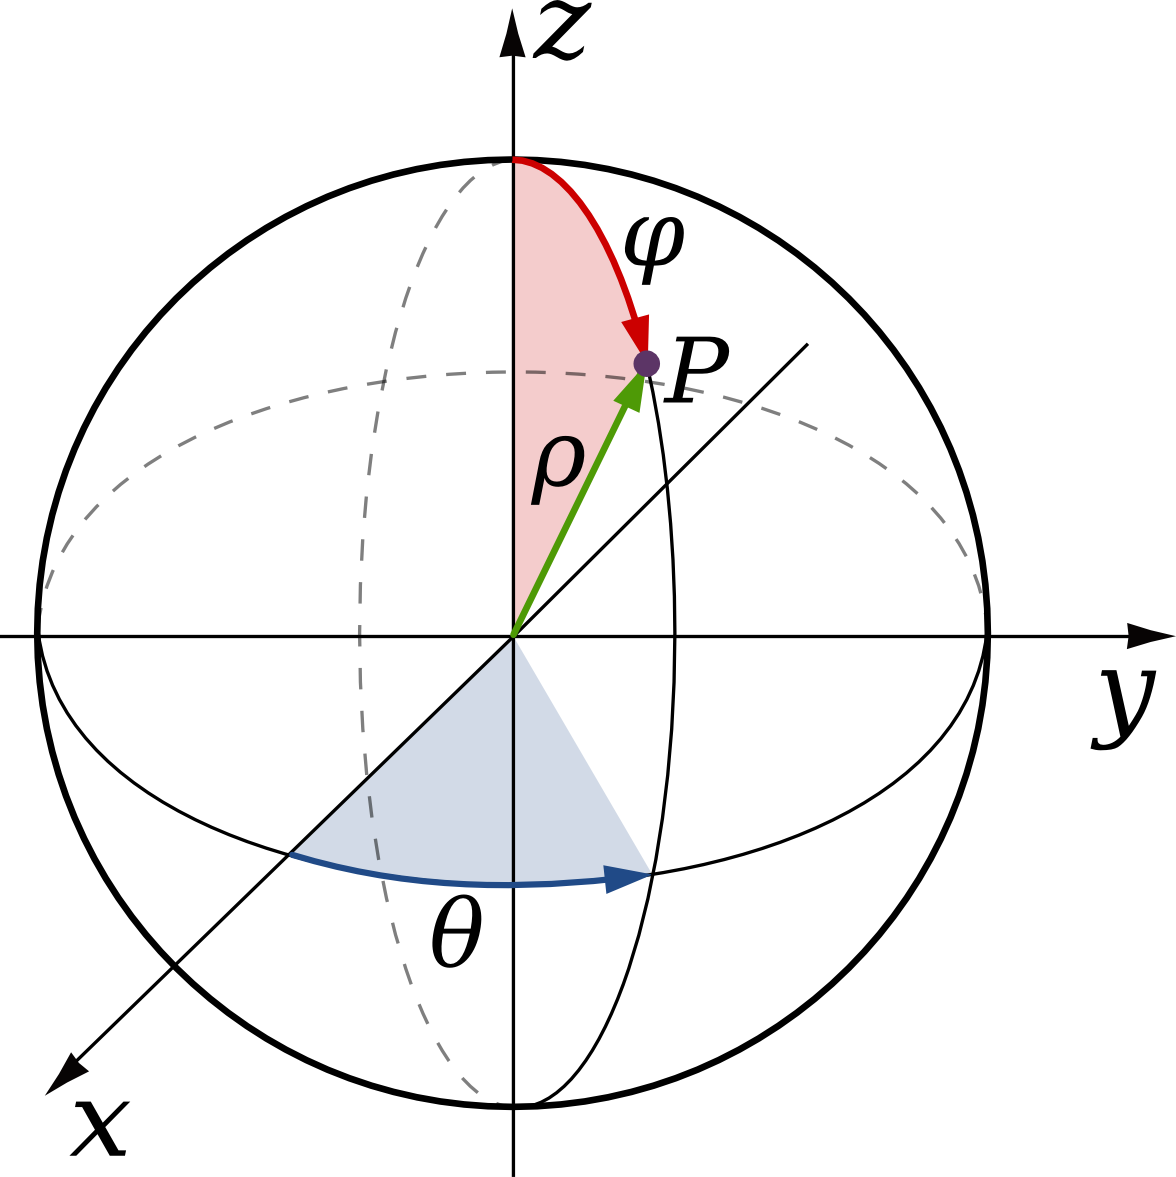
\includegraphics[width=.2\textwidth]{images/spherique}

\vspace{6cm}
\end{exemple}


\begin{exemple}
\textit{Calcul de masse d'un tore  de masse volumique $\mu$ (en $kg/m^3$).}

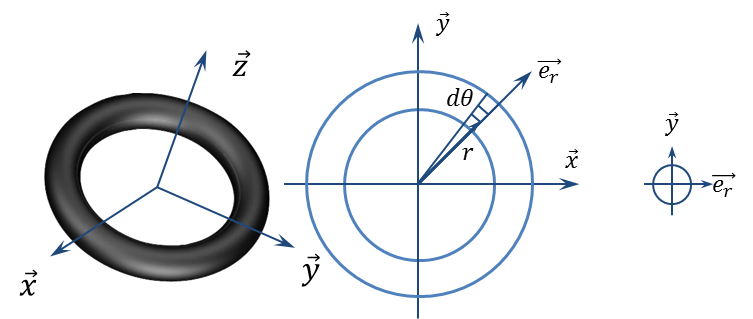
\includegraphics[width=.4\textwidth]{images/tore2}

\vspace{6cm}
\end{exemple}




\begin{exemple}
\textit{Calcul du centre de gravité d'un demi disque d'épaisseur négligeable et de masse surfacique $\mu$ (en $kg/m^2$).}

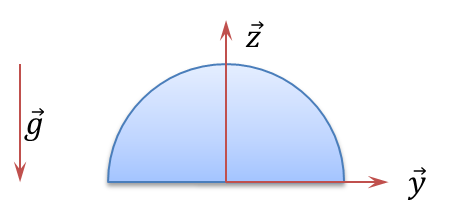
\includegraphics[width=.2\textwidth]{images/disque}

\vspace{6cm}
\end{exemple}

\section{Actions mécaniques de contact}


\subsection{Actions surfaciques}
\begin{resultat}
\textbf{Actions surfaciques}

Soit un solide $S$  (ou une partie de $S$) soumise à un champ de pression sur une surface $\mathcal{S}$.


Le vecteur densité de force est donné par : $f(M)\vect{u(M)} = p(M) \vect{n(M)}$ où $p(M)$ désigne un champ de pression (en $Pa$) et $\vect{n(M)}$ le vecteur normal à la surface au point $M$.

Au point $M$, on peut exprimer le torseur des actions mécaniques :
$$
\torseurstat{T}{\text{Pres}}{S} =
\torseurl{%
\vectf{\text{Pres}}{S}=\iint\limits_{\mathcal{S}}p(M)\vect{n}d\mathcal{S}}{%
\vectm{M}{\text{Pres}}{S}=\vect{0}}{%
M}
=
\torseurl{%
\vectf{\text{Pres}}{S}=\iint\limits_{\mathcal{S}}p(M)\vect{n}d\mathcal{S}}{%
\vectm{O}{\text{Pres}}{S}=\iint\limits_{\mathcal{S}}  \vect{OM}\wedge p(M)\vect{n}d\mathcal{S}}{%
O}
$$
n
\end{resultat}

\begin{rem}
Ce modèle permet d'exprimer :
\begin{itemize}
\item les actions mécaniques d'un fluide sur une surface (dans un vérin par exemple);
\item les actions mécaniques d'un solide sur un autre (embrayage).
\end{itemize}
\end{rem}

\begin{exemple}
\textit{Efforts transmissibles par clavette}

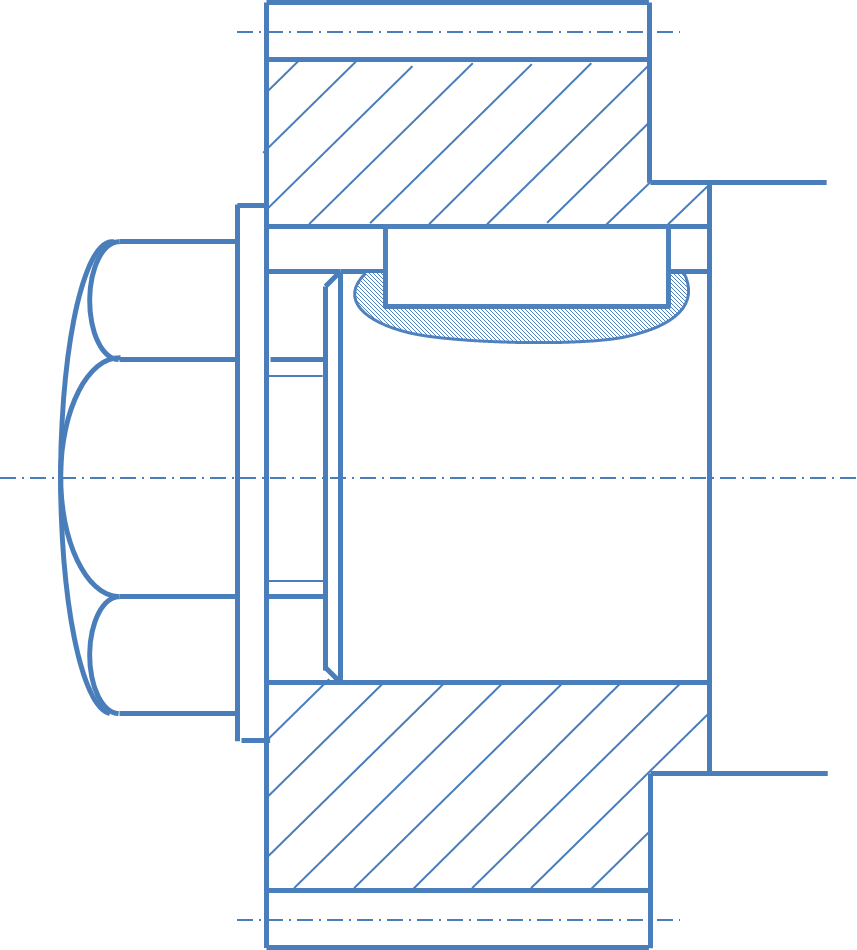
\includegraphics[width=.25\textwidth]{images/clavette}
\end{exemple}

\subsection{Torseurs d'actions mécaniques dans les liaisons cinématiques}
\begin{center}
\begin{tabular}{|p{.15\textwidth}|p{.3\textwidth}||p{.15\textwidth}|p{.3\textwidth}|}
\hline
\begin{center}
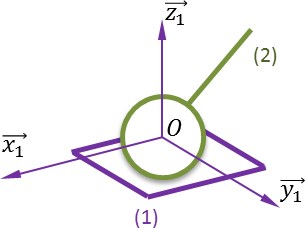
\includegraphics[height=1.5cm]{images/ponctuelle}
\textit{Liaison sphère -- plan} 
\end{center}&
$$
\torseurstat{T}{S_1}{S_2}
=\torseurcol{0}{0}{Z_{12}}{0}{0}{0}{O}
$$
&
\begin{center}
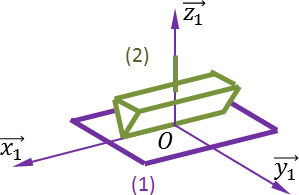
\includegraphics[height=1.5cm]{images/rectiligne}
\textit{Liaison cylindre -- plan} 
\end{center}&
$$
\torseurstat{T}{S_1}{S_2}
=\torseurcol{0}{0}{Z_{12}}{0}{M_{12}}{0}{O}
$$\\\hline
\begin{center}
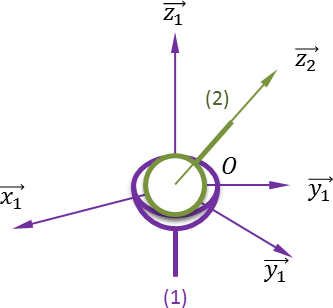
\includegraphics[height=1.5cm]{images/rotule}
\textit{Liaison rotule} 
\end{center}&
$$
\torseurstat{T}{S_1}{S_2}
=\torseurcol{X_{12}}{Y_{12}}{Z_{12}}{0}{0}{0}{O}
$$
&
\begin{center}
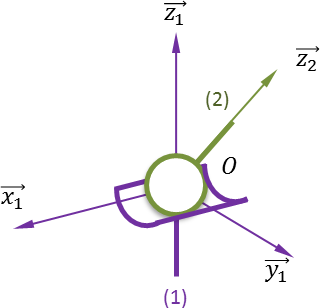
\includegraphics[height=1.5cm]{images/annulaire}
\textit{Liaison sphère -- cylindre} 
\end{center}&
$$
\torseurstat{T}{S_1}{S_2}
=\torseurcol{0}{Y_{12}}{Z_{12}}{0}{0}{0}{O}
$$\\\hline
\begin{center}
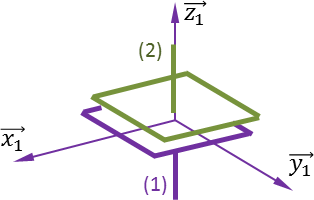
\includegraphics[height=1.5cm]{images/plan}
\textit{Liaison appui plan} 
\end{center}&
$$
\torseurstat{T}{S_1}{S_2}
=\torseurcol{0}{0}{Z_{12}}{L_{12}}{M_{12}}{0}{O}
$$
&
\begin{center}
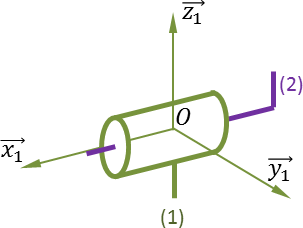
\includegraphics[height=1.5cm]{images/pivotg}
\textit{Liaison pivot glissant} 
\end{center}&
$$
\torseurstat{T}{S_1}{S_2}
=\torseurcol{0}{Y_{12}}{Z_{12}}{0}{M_{12}}{N_{12}}{O}
$$\\\hline
\begin{center}
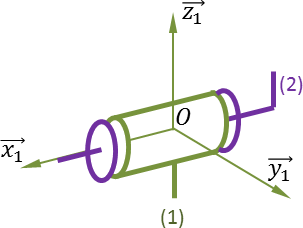
\includegraphics[height=1.5cm]{images/pivot}
\textit{Liaison pivot} 
\end{center}&
$$
\torseurstat{T}{S_1}{S_2}
=\torseurcol{X_{12}}{Y_{12}}{Z_{12}}{0}{M_{12}}{N_{12}}{O}
$$
&
\begin{center}
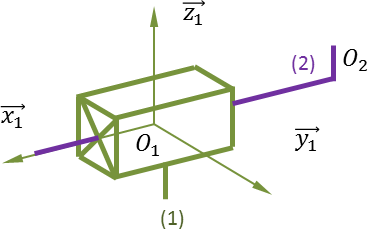
\includegraphics[height=1.5cm]{images/glissiere}
\textit{Liaison glissière} 
\end{center}&
$$
\torseurstat{T}{S_1}{S_2}
=\torseurcol{0}{Y_{12}}{Z_{12}}{L_{12}}{M_{12}}{N_{12}}{O}
$$\\\hline
\begin{center}
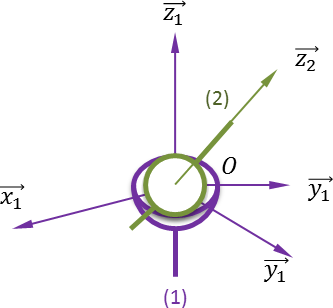
\includegraphics[height=1.5cm]{images/rotuled}
\textit{Liaison rotule à doigt} 
\end{center}&
$$
\torseurstat{T}{S_1}{S_2}
=\torseurcol{X_{12}}{Y_{12}}{Z_{12}}{0}{0}{N_{12}}{O}
$$
&
\begin{center}
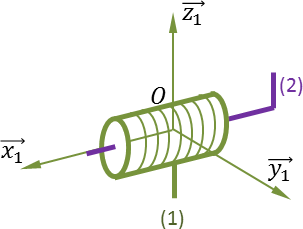
\includegraphics[height=2cm]{images/helico}
\textit{Liaison hélicoïdale} 
\end{center}&
$$
\torseurstat{T}{S_1}{S_2}
=\torseurcol{X_{12}}{Y_{12}}{Z_{12}}{L_{12}}{M_{12}}{N_{12}}{O}
$$

$$L_{12}=-X_{12}\cdot\dfrac{pas}{2\pi}$$
\\\hline
\end{tabular}
\end{center}


\subsection{Théorème de Pascal}
\begin{theo}
\begin{minipage}[c]{.5\linewidth}
\textbf{Théorème de Pascal}

Pour un fluide statique, la pression effective en u point $M$ immergé à une profondeur $h$ veut : 
$$
P(M) - P_{\text{atm}} = \mu g h
$$
On note :
\begin{itemize}
\item $P(M)$ la pression absolue au point $M$ (en $Pa$);
\item $P_{\text{atm}}$ : pression atmosphérique (en $Pa$);
\item $\mu$ : masse volumique du fluide en $kg/m^3$;
\item $h$ : profondeur du point $M$ (en $m$).
\end{itemize}
\end{minipage}\hfill
\begin{minipage}[c]{.4\linewidth}
\begin{center}
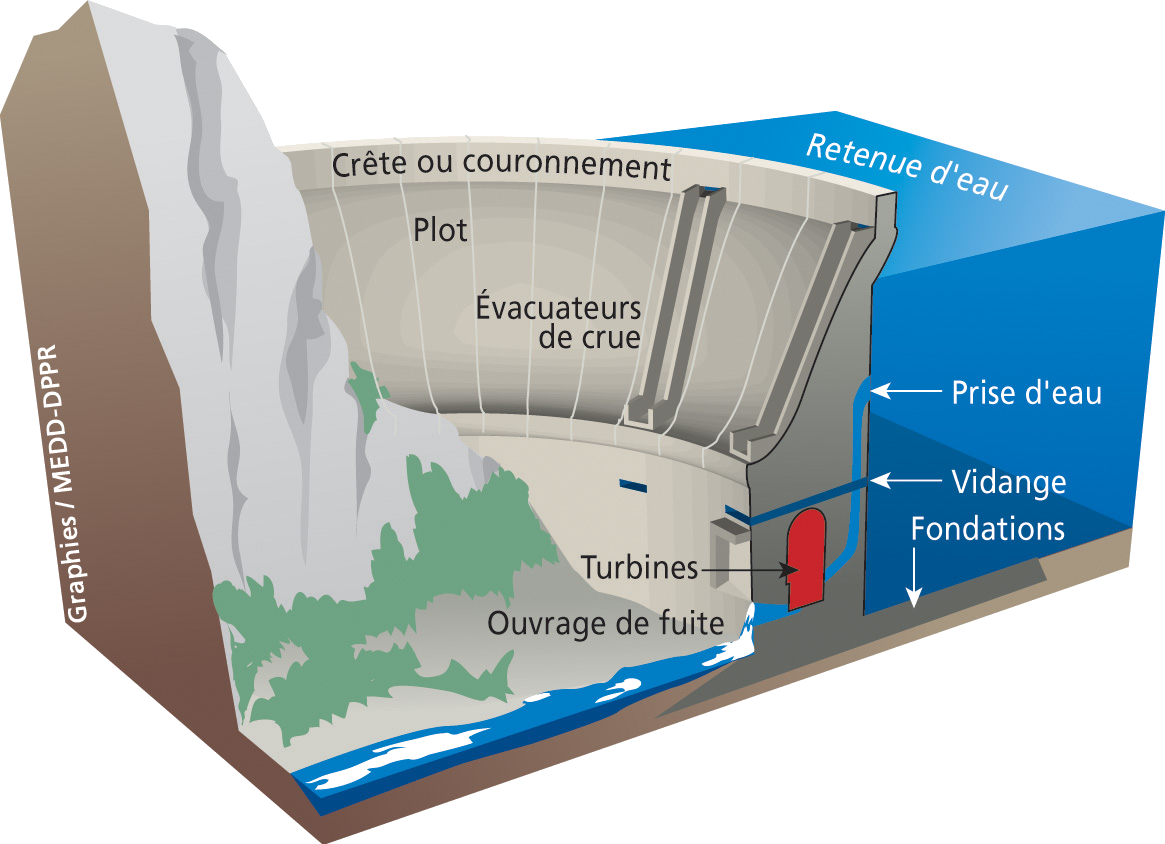
\includegraphics[width=\textwidth]{images/barrage}
\end{center}
\end{minipage}
\end{theo}

\begin{rem}
Une pression s'exprime en Pascal (Pa). 

On a  $1\; Pa = 1\; N/m^2$, $1\; MPa = 1\; N/mm^2$, $1\; bar = 10^5 \; Pa$.
\end{rem}



\subsection{Théorème d'Archimède}

\begin{theo}
\textbf{Théorème d'Archimède}

\begin{minipage}[c]{.6\linewidth}
Tout corps plongé dans un fluide reçoit de la part de celui-ci une action mécanique représentable par un glisseur :
$$
\torseurstat{T}{\text{Fluide}}{S}=
\torseurl{%
\vectf{\text{Fluide}}{S}=-m_f\vect{g}
}{%
\vect{0}
}{%
G}
$$

\begin{itemize}
\item $G$ centre d'inertie du solide (ou de l'ensemble matériel);
\item $m_f$ : masse de fluide déplacée (en $kg$);
\item $\vect{g}$ : accélération de la pesanteur (en $m/s^2$).
\end{itemize}
\end{minipage}
\begin{minipage}[c]{.35\linewidth}
\begin{center}
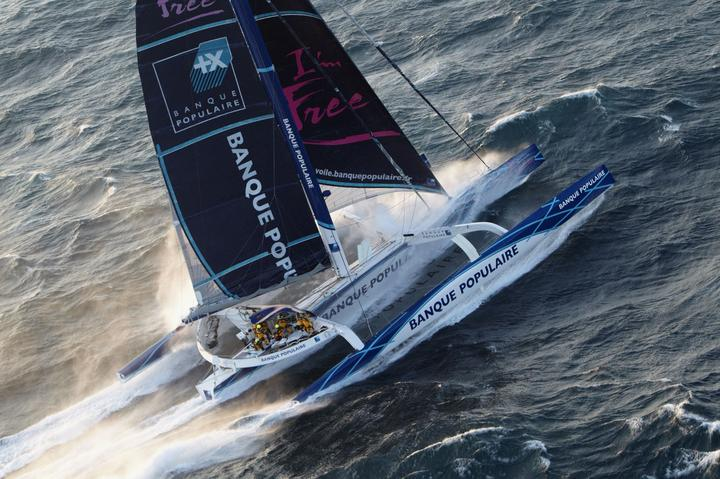
\includegraphics[width=.9\textwidth]{images/bateau}
\textit{Flottabilité d'un bateau \cite{bateau}}
\end{center}
\end{minipage}
\end{theo}
\subsection{Action transmissible par des ressorts}
\begin{resultat}
\begin{minipage}[c]{.6\linewidth}
\textbf{Ressort de compression -- traction}

Le torseur d'action d'un ressort sur un système matériel $S$ est donné par : 
$$
\torseurstat{T}{\text{Ressort}}{S} =
\torseurl{%
\vectf{\text{Ressort}}{S}=k\left(l-l_0\right)\vect{u}}{%
\vectm{A}{\text{Ressort}}{S}=\vect{0}
}{%
A}
$$
\begin{itemize}
\item $k$ : coefficient de raideur du ressort (en $N/m$);
\item $l_0$ : longueur libre (ou à vide) (en $m$);
\item $l$ : longueur en charge (en $m$).
\end{itemize}
\end{minipage} \hfill
\begin{minipage}[c]{.3\linewidth}
\begin{center}
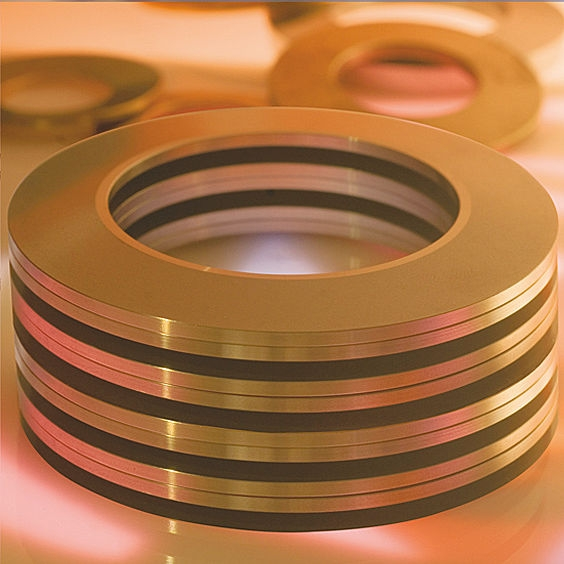
\includegraphics[width=.8\textwidth]{images/rondelles}
\textit{Rondelles de Belleville \cite{rondelles}}
\end{center}
\end{minipage}

\end{resultat}


\begin{resultat}
\begin{minipage}[c]{.6\linewidth}
\textbf{Ressort couple}

Le torseur d'action d'un ressort sur un système matériel $S$ est donné par : 
$$
\torseurstat{T}{\text{Ressort}}{S} =
\torseurl{%
\vectf{\text{Ressort}}{S}=\vect{0}}{%
\vectm{A}{\text{Ressort}}{S}=k\alpha\vect{u}
}{%
A}
$$
\begin{itemize}
\item $k$ : coefficient de raideur du ressort (en $Nm/rad$);
\item $\alpha$ : déflexion angulaire (en $rad$).
\end{itemize}
\end{minipage}\hfill
\begin{minipage}[c]{.35\linewidth}
\begin{center}
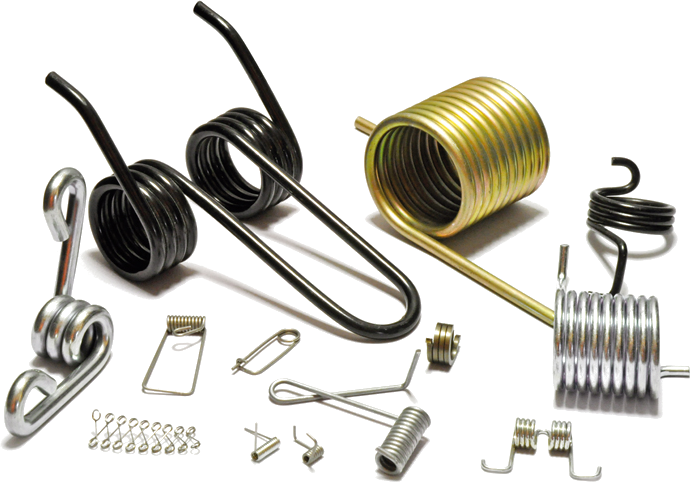
\includegraphics[width=.9\textwidth]{images/torsion}
\textit{Ressort de torsion\cite{torsion}}
\end{center}
\end{minipage}
\end{resultat}

\subsection{Actions de frottement visqueux}
\begin{theo}
\textbf{Force de frottement -- Basse vitesse -- Régime laminaire}

%\begin{minipage}[c]{.6\linewidth}
Soit un système matériel animé d'une vitesse $\vectv{C}{S}{\mathcal{R}}$. Lors de son déplacement, pour des basses vitesses et en régime laminaire, les actions du fluide sur $S$ au centre de poussée $P$ peuvent être modélisées par le torseur :
$$
\torseurstat{T}{\text{Fluide}}{S} =
\torseurl{%
\vectf{\text{Fluide}}{S}=-f_v \vectv{C}{S}{\mathcal{R}}}{%
\vectm{C}{\text{Fluide}}{S}=\vect{0}}{%
C}
$$

avec $f_v$ : frottement visqueux (en $N \cdot s \cdot m^{-1} $).

On peut considérer une vitesse faible comme étant inférieur à $5\; m/s$ dans l'air.

%\end{minipage}
%\begin{minipage}[c]{.35\linewidth}
%\begin{center}
%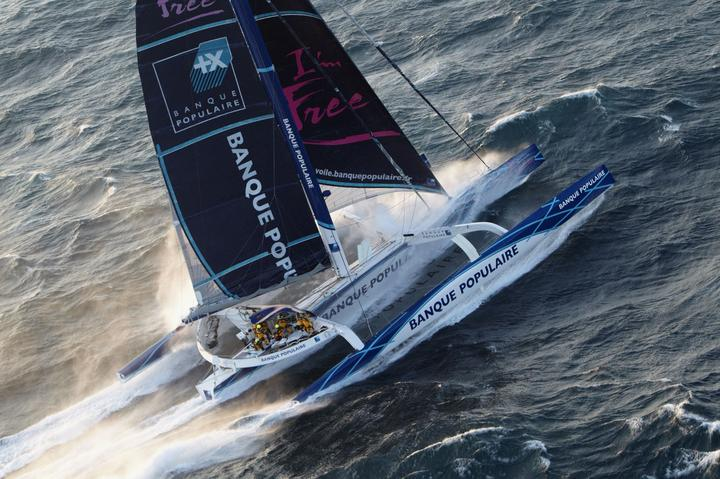
\includegraphics[width=.9\textwidth]{images/bateau}
%\end{center}
%\end{minipage}
\end{theo}


\begin{theo}
\textbf{Couple de frottement -- Basse vitesse -- Régime laminaire}

%\begin{minipage}[c]{.6\linewidth}
Soit un système matériel animé d'un taux de rotation $\vecto{S}{\mathcal{R}}=\omega \vect{z}$. Lors de sa rotation, pour des basses vitesses, le couple de frottement peut être modélisé par le torseur ($A$ est un point appartenant à l'axe de rotation):
$$
\torseurstat{T}{\text{Fluide}}{S} =
\torseurl{%
\vectf{\text{Fluide}}{S}=\vect{0}}{%
\vectm{A}{\text{Fluide}}{S}=-f_v \vecto{S}{\mathcal{R}}}{%
A}
$$

avec $f_v$ : frottement visqueux (en $N \cdot m \cdot s \cdot rad^{-1} $).

%\end{minipage}
%\begin{minipage}[c]{.35\linewidth}
%\begin{center}
%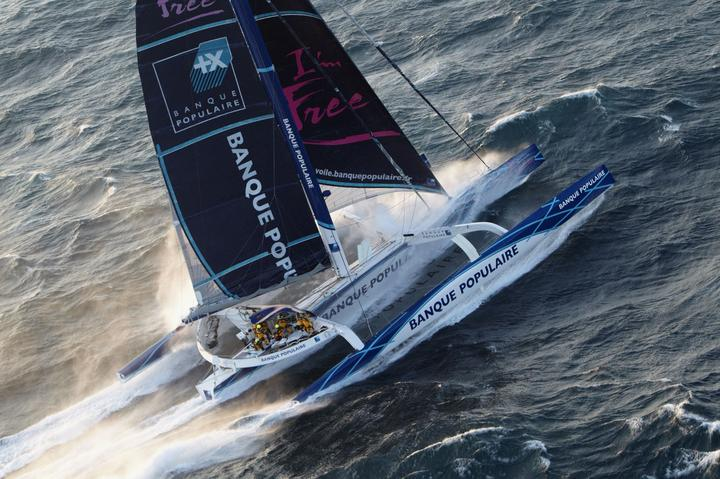
\includegraphics[width=.9\textwidth]{images/bateau}
%\end{center}
%\end{minipage}
\end{theo}



\begin{theo}
\textbf{Force de frottement -- Vitesse moyenne -- Régime turbulent}

%\begin{minipage}[c]{.6\linewidth}
Soit un système matériel animé d'une vitesse $\vectv{C}{S}{\mathcal{R}}$ de vecteur directeur $\vect{u}$. Lors de son déplacement, les actions du fluide sur $S$ au centre de poussée $P$ peuvent être modélisées par le torseur :
$$
\torseurstat{T}{\text{Fluide}}{S} =
\torseurl{%
\vectf{\text{Fluide}}{S}=-C_x \dfrac{1}{2} \rho S \vectv{C}{S}{\mathcal{R}}^2 \vect{u}}{%
\vectm{C}{\text{Fluide}}{S}=\vect{0}}{%
C}
$$

avec :
\begin{itemize}
\item $C_x$ : coefficient de traînée caractérisant la géométrieu du solide (sans unité);
\item $\rho$ : masse volumique du fluide ($kg/m^3$);
\item $S$ : aire du solide selon la direction perpendiculaire à la vitesse (en $m^2$);
\end{itemize}

On peut considérer une moyenne faible comme étant inférieur entre 5 et 20 $m/s$ dans l'air.

%\end{minipage}
%\begin{minipage}[c]{.35\linewidth}
%\begin{center}
%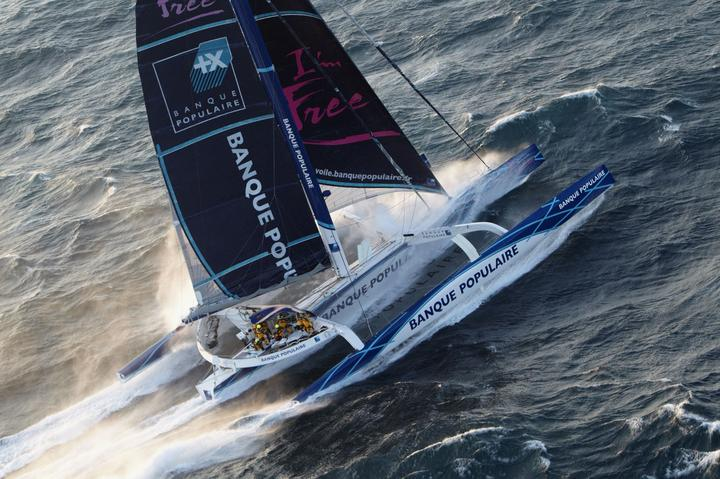
\includegraphics[width=.9\textwidth]{images/bateau}
%\end{center}
%\end{minipage}
\end{theo}

%\section{Action mécanique transmissible par contact entre pièce}

%\section{Action mécanique transmissible par les liaisons cinématiques}

\newpage


\section{Étude locale du contact entre pièces}

\begin{hypo}
On considèrera que : 
\begin{itemize}
\item les pièces sont considérées indéformables;
\item la résistance au roulement et au pivotement sont négligées (voir définition dans le cours de cinématique).
\end{itemize}
\end{hypo}

On rappelle que le torseur des actions transmissibles est donné par :
$$
\torseurstat{T}{\text{ext}}{S}=
\torseurl{%
\vect{R_{(\text{ext}\rightarrow S)}} 
= \iint\limits_{\mathcal{S}} f(M) \vect{u(M)} d\mathcal{S}}{%
\vectm{P}{\text{ext}}{S} = \iint\limits_{\mathcal{S}}\vect{PM}\wedge d\vectf{\text{ext}}{S}}{P}
$$

$f(M) \cdot \vect{u(M)}$ désigne le vecteur densité d'effort. 


\subsection{Cas du contact ponctuel}

\subsubsection{Modèle sans frottement}
\begin{resultat}
\begin{minipage}[c]{.6\linewidth}
Dans le cas d'un contact ponctuel en $I$ et de normale $\vect{n_{21}}$, le torseur d'action mécanique de la pièce $S_2$ sur $S_1$ est donné par :
$$
\torseurstat{T}{S_2}{S_1}=
\torseurl{% 
\vectf{S_2}{S_1}=  ||\vectf{S_2}{S_1}|| \vect{n_{21}}}{%
\vectm{I}{S_2}{S_1} =\vect{0}}{I}
$$
\end{minipage}\hfill
\begin{minipage}[c]{.35\linewidth}
\begin{center}
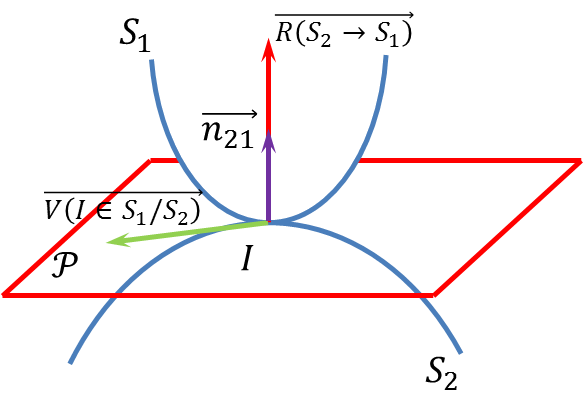
\includegraphics[width=\textwidth]{images/cp}
\end{center}
\end{minipage}
\end{resultat}

\subsubsection{Modèle avec frottement -- Modèle de Coulomb}
\begin{theo}
\textbf{Glissement}


On considère un contact ponctuel en $I$ et de normale $\vect{n_{21}}$. $\vectv{I}{S_1}{S_2}$ est la vitesse de glissement entre les solides. $\vectv{I}{S_1}{S_2}$ appartient au plan $\mathcal{P}$ tangent entre les deux solides.

On se place dans le cas où la vitesse de glissement est non nulle :
$$\vectv{I}{S_1}{S_2}\neq \vect{0}$$

\begin{minipage}[c]{.6\linewidth}

Dans ce cas, $\vectf{S_2}{S_1}$ se décompose en un effort normal $\vect{N\left(S_2\rightarrow S_1\right)}$ suivant le vecteur $\vect{n_{21}}$ et un effort tangentiel $\vect{T\left(S_2\rightarrow S_1\right)}$ appartenant au plan $\mathcal{P}$.

On a alors :
$$
\vectf{S_2}{S_1} = \vect{N\left(S_2\rightarrow S_1\right)}+\vect{T\left(S_2\rightarrow S_1\right)}
$$ 

Par ailleurs, en notant $f$ le facteur de frottement entre les deux solides, on a la relation suivante :
$$
||\vect{T\left(S_2\rightarrow S_1\right)}|| = f\cdot ||\vect{N\left(S_2\rightarrow S_1\right)}||
$$

Enfin, le vecteur tangentiel $\vect{T\left(S_2\rightarrow S_1\right)}$ s'oppose au vecteur $\vectv{I}{S_1}{S_2}$
\end{minipage}\hfill
\begin{minipage}[c]{.35\linewidth}
\begin{center}
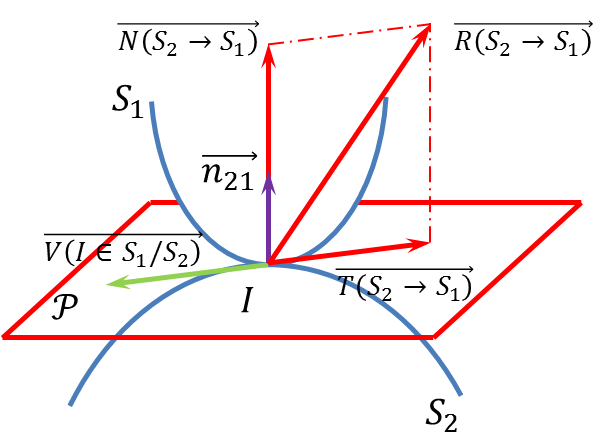
\includegraphics[width=\textwidth]{images/coulomb}
\end{center}
\end{minipage}
\end{theo}

\begin{theo}
\textbf{Adhérence}

On se place dans le cas où la vitesse de glissement est nulle :
$$\vectv{I}{S_1}{S_2} = \vect{0}$$

On note $\mu$ le facteur d'adhérence entre les deux matériaux. On a alors : 
$$
||\vect{T\left(S_2\rightarrow S_1\right)}|| \leq \mu\cdot ||\vect{N\left(S_2\rightarrow S_1\right)}||
$$
\end{theo}


\subsubsection{Interprétation graphique}
\begin{minipage}[c]{.6\linewidth}
Suivant la direction de la vitesse de glissement, l'effort $\vectf{S_2}{S_1}$ décrit donc un cône de sommet $I$ et de demi-angle au sommet $\varphi$.
\end{minipage}\hfill
\begin{minipage}[c]{.35\linewidth}
\begin{center}
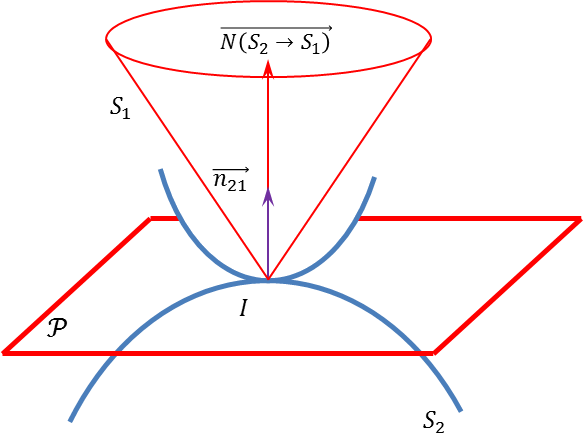
\includegraphics[width=\textwidth]{images/cone}
\end{center}
\end{minipage}

Lorsqu'il y a \textbf{glissement}, l'effort $\vectf{S_2}{S_1}$ est situé \textbf{sur} le cône de frottement. 

Lorsqu'il y a \textbf{adhérence}, l'effort $\vectf{S_2}{S_1}$ est situé \textbf{dans} le cône de révolution.  \textbf{La direction de l'effort n'est donc pas connue, \textit{a priori}.}

\begin{rem}
\begin{minipage}[c]{.4\linewidth}
Dans le cas du glissement, en redessinant les efforts et en utilisant la relation de Coulomb, on a donc :
$$
f = \tan\varphi
$$
\end{minipage}\hfill
\begin{minipage}[c]{.4\linewidth}
\begin{center}
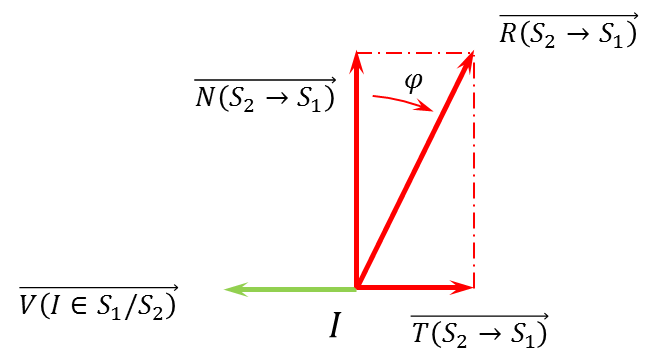
\includegraphics[width=\textwidth]{images/tanphi}
\end{center}
\end{minipage}
\end{rem}

\subsection{Cas général}
\begin{theo}
\textbf{Torseur d'action mécanique transmise par contact avec frottement}

$$
\torseurstat{T}{S_2}{S_1}=
\torseurl{%
\vect{R_{(ext\rightarrow S)}} 
= \iint\limits_{\mathcal{S}} f(M) \vect{u(M)} d\mathcal{S}}{%
\vectm{P}{ext}{S} = \iint\limits_{\mathcal{S}}\vect{PM}\wedge d\vectf{ext}{S}}{M}
$$

On a alors :
$$
f(M) \vect{u(M)} = p_{21}(M)\vect{n_{21}}+\vect{\tau_{21}}(M)
$$
Dans le cas du glissement :
$$||\vect{\tau_{21}}(M)||=p_{21}\cdot f$$
En notant : 
\begin{itemize}
\item $p_{21}(M)$ pression de contact au point $M$ (en $N/m^2$);
\item $\vect{\tau_{21}}(M)$ : la projection tangentielle de la densité surfacique (norme en $N/m^2$);
\item $f$ facteur de frottement.
\end{itemize}
\end{theo}

\subsubsection{Exemple : Couple transmis par frottement dans un embrayage à disque}

\begin{minipage}[c]{.3\linewidth}
\begin{center}
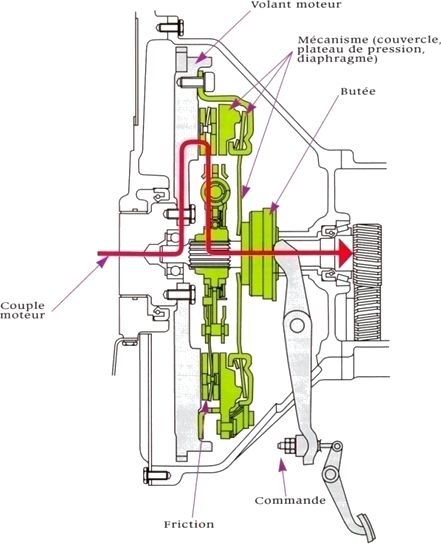
\includegraphics[width=.95\textwidth]{images/embrayage}
\end{center}
\end{minipage}\hfill
\begin{minipage}[c]{.65\linewidth}
\begin{center}
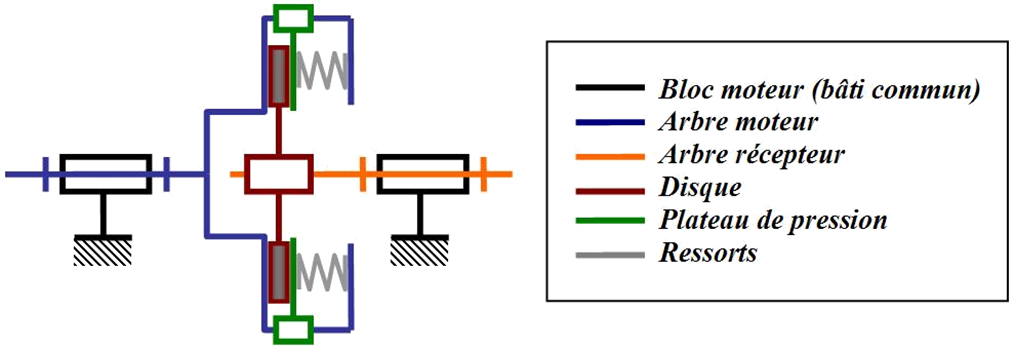
\includegraphics[width=.95\textwidth]{images/embrayage2}
\end{center}
\end{minipage}

\begin{exemple}
On donne $k$ la raideur des ressorts, $f$ le facteur de frottement entre les le disque et l'arbre moteur, $r$ le petit rayon de la couronne et $R$ le grand rayon de la couronne. Calculer le couple transmissible par adhérence entre l'arbre moteur et le disque. On fera l'hypothèse que l'action créée par les ressorts sur le plateau de compression est uniforme. 

\textbf{Expression du couple infinitésimal}
$$
d\vectm{\text{Plateau}}{\text{Disque}}{O} =
d\vectm{P}{D}{O} =  \vect{OM}\wedge d\vectf{P}{D}
$$

\textbf{Expression de la résultante infinitésimale}

$$
d\vectf{P}{D} = d\vect{N(P\rightarrow D)}+d\vect{T(P\rightarrow D)}
$$

\textbf{Expression de l'effort normal}

$$
d\vect{N(P\rightarrow D)} = p \vect{n} d\mathcal{S} = -p \vect{z} d\mathcal{S}
$$

\textbf{Expression de l'unité de surface}

$$
d\mathcal{S} = \rho d\theta d\rho
$$

\textbf{Expression de l'effort tangentiel}

D'après le modèle de Coulomb, on commence par identifier le vecteur $\vectv{M}{D}{P}$.
Le vecteur tangentiel est donc opposé à ce dernier. A la limite du glissement on a alors : 
$$
d\vect{T(P\rightarrow D)} = -f ||d\vect{N(P\rightarrow D)}|| \vect{v}    = fp d\mathcal{S}\vect{v}
$$

\textbf{Calcul final}

On note $\vect{OM}=\rho\vect{u}$ :

\begin{eqnarray*}
\vectm{O}{P}{D}  
&=& d\vectm{O}{P}{D}  \\
&=& \int \vect{OM}\wedge d\vectf{P}{D} \\
&=& \int \rho\vect{u} \wedge \left( d\vect{N(P\rightarrow D)}+d\vect{T(P\rightarrow D)} \right)\\
&=& \int \rho\vect{u} \wedge \left( -p \vect{z} d\mathcal{S} +fp d\mathcal{S}\vect{v} \right)\\
&=& \iint p\rho\vect{v} d\mathcal{S} +\iint pf\rho  \vect{z}d\mathcal{S} = 
\iint p\rho\vect{v} \rho d\theta d\rho +\iint pf\rho  \vect{z}\rho d\theta d\rho \\
\end{eqnarray*}

\begin{eqnarray*}
\iint p\rho\vect{v} \rho d\theta d\rho = \iint p\rho\left(\cos\theta\vect{y}-\sin\theta\vect{x} \right) \rho d\theta d\rho \\
=\iint p\rho\cos\theta\vect{y}  \rho d\theta d\rho-\iint p\rho \sin\theta\vect{x}  \rho d\theta d\rho \\
=p \vect{y}  \int\limits_{r}^{R} \int\limits_{0}^{2\pi}\cos\theta d\theta \rho^2 d\rho- p\vect{x}\int\limits_{r}^{R} \int\limits_{0}^{2\pi} \sin\theta  \rho^2 d\theta d\rho \\
=p \left[ \sin\theta\right]_{0}^{2\pi}\left[ \dfrac{1}{3}\rho^3\right]_{r}^{R}\vect{y}\
 -
p \left[ -\cos\theta\right]_{0}^{2\pi}\left[ \dfrac{1}{3}\rho^3\right]_{r}^{R}\vect{x} = \vect{0}
\end{eqnarray*}

\begin{eqnarray*}
\iint pf\rho^2 \vect{z} d\theta d\rho =
pf \left[ \theta\right]_{0}^{2\pi}\left[ \dfrac{1}{3}\rho^3\right]_{r}^{R} \vect{z}\\
= pf2\pi \dfrac{R^3-r^3}{3} 
\end{eqnarray*} 

Enfin, en notant $F_r$ l'effort (uniformément réparti) exercé par le ressort sur toute la couronne, on a donc :
$$
p=\dfrac{F_r}{\pi \left(R^2-r^2 \right)}
$$

Au final : 

$$ \vectm{O}{P}{D}  
= f\dfrac{2}{3} \dfrac{R^3-r^3}{R^2-r^2} F_r
$$
\end{exemple}
\subsection{Notions de tribologie}

\subsubsection{Facteur de frottement et de glissement}
Le facteur de frottement dépend : 
\begin{itemize}
\item de la nature des matériaux en contact; 
\item de la rugosité des surfaces de contact; 
\item de la présence ou non de lubrifiant.
\end{itemize}

Le facteur de frottement ne dépend pas de la pression de contact entre deux solides.

\begin{center}
\begin{tabular}{|c||c|c||c|c|}
\hline
\multirow{2}{*}{Matériaux} 
& \multicolumn{2}{c||}{Facteur d'adhérence} & \multicolumn{2}{c|}{Facteur de glissement} \\
\cline{2-5}
& Sec & Lubrifié & Sec & Lubrifié \\
\hline
\hline
Acier / Acier & 0,2 à 0,3 & 0,15 à 0,2 & 0,2 & 0,12 \\ \hline
Acier / Fonte & 0,2 & 0,12 à 0,2 & 0,15 & 0,08 \\ \hline
Acier / Bronze & 0,2 & 0,15 à 0,2 & 0,2 & 0,12 \\ \hline
Acier / Métal fritté &  & 0,1 à 0,18 & 0,1 à 0,12 & 0,03 à 0,06 \\ \hline
Acier / Garniture de friction & 0,3 à 0,4 &  & 0,25 à 0,35 &  \\ \hline
Acier / Graphite &  & 0,1 &  & 0,09 \\ \hline
Acier / Palier PTFE & 0,08 à 0,4 &  & 0,02 à 0,08 & 0,003 à 0,05 \\ \hline
Pneu neuf / Route & 1 & 0,6  & 0,5 à 0,6  & 0,2 à 0,5\\ \hline
\end{tabular}
\end{center}
%\subsubsection{Détermination expérimentale du coefficient de frottement}

\begin{thebibliography}{2}
\bibitem{millau1}{\url{http://cnrsm.creteil.iufm.fr/g01_dp/viaduc_millau_apk_44/01_greish/06_instrumentation_millau_final_otua.pdf}.}
\bibitem{verin}{\url{http://maaon.free.fr/articles/?page_id=2}.}
\bibitem{zerog}{\url{http://3.bp.blogspot.com/-Nv8wocGYY9w/Td2EzuOWTKI/AAAAAAAAArw/Fsn1MvhEWDQ/s1600/airbus_zero_G_1.jpg}.}
\bibitem{bateau}{\url{http://www.voile.banquepopulaire.fr/pics/9/1044/3e40b1889ec5435595b93795554ceb69.jpg}.}
\bibitem{rondelles}{\url{http://www.directindustry.fr/prod/borrelly/rondelles-elastiques-belleville-50471-343362.html}.}
\bibitem{torsion}{\url{http://www.hellopro.fr/images/produit-2/0/2/5/ressort-de-torsion-259520.jpg}.}
%\bibitem{pomme}{http://fabrice.sincere.free.fr/qcm/image/Newton_Gotlib.jpg}
\end{thebibliography}


\end{document}


